








\usepackage{xstring}
\usepackage{graphicx}
\usepackage{hyperref}

%%
%% This is file `sample-manuscript.tex',
%% generated with the docstrip utility.
%%
%% The original source files were:
%%
%% samples.dtx  (with options: `manuscript')
%% 
%% IMPORTANT NOTICE:
%% 
%% For the copyright see the source file.
%% 
%% Any modified versions of this file must be renamed
%% with new filenames distinct from sample-manuscript.tex.
%% 
%% For distribution of the original source see the terms
%% for copying and modification in the file samples.dtx.
%% 
%% This generated file may be distributed as long as the
%% original source files, as listed above, are part of the
%% same distribution. (The sources need not necessarily be
%% in the same archive or directory.)
%%
%% Commands for TeXCount
%TC:macro \cite [option:text,text]
%TC:macro \citep [option:text,text]
%TC:macro \citet [option:text,text]
%TC:envir table 0 1
%TC:envir table* 0 1
%TC:envir tabular [ignore] word
%TC:envir displaymath 0 word
%TC:envir math 0 word
%TC:envir comment 0 0
%%
%%
%% The first command in your LaTeX source must be the \documentclass command.
\documentclass[manuscript,screen,review]{acmart}

%%
%% \BibTeX command to typeset BibTeX logo in the docs
\AtBeginDocument{%
  \providecommand\BibTeX{{%
    \normalfont B\kern-0.5em{\scshape i\kern-0.25em b}\kern-0.8em\TeX}}}

%% Rights management information.  This information is sent to you
%% when you complete the rights form.  These commands have SAMPLE
%% values in them; it is your responsibility as an author to replace
%% the commands and values with those provided to you when you
%% complete the rights form.
\setcopyright{acmlicensed}
\copyrightyear{2018}
\acmYear{2018}
\acmDOI{XXXXXXX.XXXXXXX}

%% These commands are for a PROCEEDINGS abstract or paper.
\acmConference[Conference acronym 'XX]{Make sure to enter the correct
  conference title from your rights confirmation emai}{June 03--05,
  2018}{Woodstock, NY}
\acmISBN{978-1-4503-XXXX-X/18/06}


%%
%% Submission ID.
%% Use this when submitting an article to a sponsored event. You'll
%% receive a unique submission ID from the organizers
%% of the event, and this ID should be used as the parameter to this command.
%%\acmSubmissionID{123-A56-BU3}

%%
%% For managing citations, it is recommended to use bibliography
%% files in BibTeX format.
%%
%% You can then either use BibTeX with the ACM-Reference-Format style,
%% or BibLaTeX with the acmnumeric or acmauthoryear sytles, that include
%% support for advanced citation of software artefact from the
%% biblatex-software package, also separately available on CTAN.
%%
%% Look at the sample-*-biblatex.tex files for templates showcasing
%% the biblatex styles.
%%

%%
%% The majority of ACM publications use numbered citations and
%% references.  The command \citestyle{authoryear} switches to the
%% "author year" style.
%%
%% If you are preparing content for an event
%% sponsored by ACM SIGGRAPH, you must use the "author year" style of
%% citations and references.
%% Uncommenting
%% the next command will enable that style.
%%\citestyle{acmauthoryear}

%%
%% end of the preamble, start of the body of the document source.
\begin{document}

%%
%% The "title" command has an optional parameter,
%% allowing the author to define a "short title" to be used in page headers.
\title{Design and Gamification for Mental Health App Engagement}

%%
%% The "author" command and its associated commands are used to define
%% the authors and their affiliations.
%% Of note is the shared affiliation of the first two authors, and the
%% "authornote" and "authornotemark" commands

\author{Vaibhav Chopra}
\affiliation{%
 \institution{Indraprastha Institute Of Technology, Delhi}
 \country{India}}

 
\author{Tejus Madan}
\affiliation{%
 \institution{Indraprastha Institute Of Technology, Delhi}
 \country{India}}


\author{Shamik Sinha}
\affiliation{%
 \institution{Indraprastha Institute Of Technology, Delhi}
 \country{India}}


%%
%% By default, the full list of authors will be used in the page
%% headers. Often, this list is too long, and will overlap
%% other information printed in the page headers. This command allows
%% the author to define a more concise list
%% of authors' names for this purpose.
\renewcommand{\shortauthors}{Trovato and Tobin, et al.}

%%
%% The abstract is a short summary of the work to be presented in the
%% article.
\begin{abstract}
Millions of individuals are affected by conditions such as anxiety, depression, and stress. While there are numerous mental support apps available, all of them struggle with user retention and motivation. To address these challenges, we propose the development of a gamified mental health app aimed at promoting emotional well-being and providing accessible support to users.
\\
The proposed app will use gamification techniques to enhance user engagement and motivation in managing their mental health. In addition to gamified elements, the app will offer therapy services delivered by qualified professionals through both online and offline sessions. Users will have the flexibility to choose from a range of therapy options, including chat, audio, and video sessions, tailored to their individual needs and preferences. The app will also provide access to supportive communities, resources, and educational content to foster a sense of connection, understanding, and empowerment among users.
\\
To ensure the effectiveness and relevance of the app, a comprehensive research and requirements-gathering process was undertaken. This included conducting interviews with a diverse sample of individuals. Additionally, an extensive review of academic literature, commercial products, and competitive analysis was conducted to gather insights into existing mental health solutions and identify areas for improvement.

\end{abstract}

%%
%% The code below is generated by the tool at http://dl.acm.org/ccs.cfm.
%% Please copy and paste the code instead of the example below.
%%
\begin{CCSXML}
<ccs2012>
 <concept>
  <concept_id>10003120.10003130.10003131</concept_id>
  <concept_desc>Human-centered computing~Collaborative and social computing systems and tools</concept_desc>
  <concept_significance>500</concept_significance>
 </concept>
 <concept>
  <concept_id>10003120.10003130.10003131</concept_id>
  <concept_desc>Human-centered computing~Interactive systems and tools</concept_desc>
  <concept_significance>300</concept_significance>
 </concept>
 <concept>
  <concept_id>10003120.10003130.10003131</concept_id>
  <concept_desc>Human-centered computing~User studies</concept_desc>
  <concept_significance>100</concept_significance>
 </concept>
 <concept>
  <concept_id>10003120.10003130.10003131</concept_id>
  <concept_desc>Human-centered computing~HCI theory, concepts and models</concept_desc>
  <concept_significance>100</concept_significance>
 </concept>
</ccs2012}
\end{CCSXML}

\ccsdesc[500]{Human-centered computing~Collaborative and social computing systems and tools}
\ccsdesc[300]{Human-centered computing~Interactive systems and tools}
\ccsdesc{Human-centered computing~User studies}
\ccsdesc[100]{Human-centered computing~HCI theory, concepts and models}


\received{20 February 2007}
\received[revised]{12 March 2009}
\received[accepted]{5 June 2009}

%%
%% This command processes the author and affiliation and title
%% information and builds the first part of the formatted document.
\maketitle

% \section{Abstract}

\section{Motivation}
According to the World Health Organization \cite{WHOmentalhealth} (2022), Mental health is defined as the state of mental well-being when individuals effectively manage the challenges faced in daily life, recognise their capabilities, thrive, and make meaningful contributions to their communities. 

In recent years, people have become increasingly aware of the importance of mental health as a part of an individual's overall state of well-being. Along with it, the development of digital interventions to support individuals has also boomed. However, there still exists a significant gap between those who receive adequate mental health support and those who require it. According to the most recent national mental health survey, over 150 million Indians need mental health support. However, only 30 million people seek care \cite{Gautham2020}. Garg et al. \cite{Garg19} (2019) also suggests, there is a scarcity of mental health professionals, which, when coupled with people's reluctance to seek help, underscores the need for improved digital solutions that engage users.


\section{Problem Statement and Vision}

Our preliminary exploratory research leads us to believe that many existing technological solutions to the issues people face with mental health lack user retention. Many mental health apps are not based on concrete empirical research and a lot of them don’t follow user-centric interaction design principles \cite{Balcombe2022}.

Through personas and scenarios, we aim to gauge motivations and pain points, mapping out a comprehensive picture of the problem. The end goal of this project is to design for a smooth user experience, taking inspiration from research-based principles such as gamification. Even at a rudimentary stage of research gamification shows a lot of promise by enhancing engagement, fun and interactivity Citation1 and we intend to delve deeper.

In the future, Mental health apps may have an important role to play in the evolution of traditional treatment and mental healthcare practices. This is primarily because the increasing democratization of technology will help combat the stigma associated with mental health issues \cite{IGIGlobal}.
 
\section{Proof of Significance}
Even though Mental health apps have been shown to be as effective as traditional mental services in improving mental health conditions like depression and anxiety, the engagement with these technologies is a big issue, and is typically way lower than traditional services \cite{Borghouts21}. Several studies have shown that these apps lose most of their users within the first two weeks after installation \cite{Auf21}. Furthermore, 74\% of users stop engaging with a health app after only 10 uses. In the top installed mental health apps on the app store, data analysis of user engagement data shows that the median of user-retention for the days 1,3 and 7 were respectively 50\% , 14.5\% , and 7\% \cite{Auf21}. Long-term engagement is especially difficult for these apps, due to the decreased motivation being a core feature of many mental illnesses such as depression and schizophrenia \cite{Torous18}.
\\
A mental app needs some form of dynamic sustainable engagement with a user to provide effective mental health services. This can be done by gamification of the app. Gamification uses the user’s voluntary interaction with the system and its affordances to promote the user in a series of psychological outcomes, such as enhanced motivation and engagement, with the final aim of shaping his/her behaviors \cite{Bitrian21}.

\section{Literature Review}
\textit{\textbf{Problem Statement} - How can user-centric design choices and gamification elements be effectively integrated into a mental health application to improve user retention and engagement, addressing the gap between individuals seeking mental health support and those requiring it?}
\\\\
During a time of constant, fast-paced technological progress, we find ourselves in a new era that has seen a phenomenal rise in mental health awareness. Furthermore, while mental health has gained a lot of attention, there is still a considerable gap in the number of health professionals available to serve the needs of those who need it, as Garg et al. \cite{Garg19} (2019) pointed out. Digital interventions have therefore become instrumental in addressing the growing demand for accessible mental health support \cite{Borghouts21}. Better known as Digital mental health interventions (DMHIs). DMHIs are technologies that provide mental health support to people through various means such as mobile apps, virtual reality platforms or internet websites. Mental health applications, in particular, have emerged as promising tools for delivering convenient and personalized interventions to individuals while ensuring the cost to achieve this is minimal  \cite{Baumel19}. However, the effectiveness and impact of such interventions are limited by their inability to engage users successfully for longer durations or before any notable changes may be observed \cite{Eysenbach05, Christensen06}.
\\ \\
Therefore, despite the proliferation of mental health applications, a significant challenge persists, i.e. user engagement and retention. Torous et al. \cite{Torous18} (2018) pointed out that while these applications hold immense potential for improving mental well-being, many users disengage from them shortly after initial use, limiting the impact and effectiveness of these interventions. Some of the reasons why users engaged in this behavior were the poor user-centric design of the application and the fact that the applications were not perceived to be trustworthy, among other things. This phenomenon of "Low Engagement" was not just limited to mental health applications but has also affected and still affects both traditional and computerized therapies for mental disorders \cite{Torous18}. Data from a market research study suggested that about 25\% of users abandon or uninstall an application just after one use \cite{AppUninstall}. Achieving Long-term engagement is therefore even more difficult. As an example, a study of an app to track asthma symptoms successfully enrolled nearly 8000 participants. Only 175 participants out of 8000 had engaged enough with the app in order to take a survey at the end of 6 months, which is just a minuscule 2\% (Chan et al., 2017, as cited in Torous et al.,2018) \cite{Torous18}.
\\ \\ 
The issue of low engagement is a complex issue to solve, and many factors are at play here. There is no one-stop solution to this problem. However, a step in the right direction would be focusing on the user interface design of the applications. User-centric design principles need to be incorporated into the development process. This approach will help us prioritize users' needs, preferences, and experiences, aiming to create intuitive, accessible, and engaging interfaces \cite{Vial22}. Unfortunately, many mental health applications have failed to adhere to these principles, resulting in interfaces that are cumbersome, unintuitive, or unappealing to users. Our goal should be to involve end users in the conception, design, and testing of apps. Bitriån et al \cite{Bitrian21} (2022) claimed close collaboration with the community to learn their needs and formulate how an app may even be useful would allow us to gauge better users' preferences and behaviors to create products that meet their expectations and enhance their experience
\\ \\
Many innovative solutions have been developed in the domain of user-centered design better to serve the needs and expectations of the people. One such approach that started gaining traction in the field, a few years ago, was integrating game-playing elements into applications. Also known as Gamification, it is described as the application of game design principles outside of gaming environments. A great example of an application that utilized principles of Gamification is Duolingo. It is a language learning app that awards points, levels, and virtual rewards for completing lessons and practicing regularly. An engaging feature it uses is the daily streak, where users can increase the streak they have held on the app by practicing and completing lessons regularly. This gives the users a sense of achievement and encourages them to continue practicing. Users earn experience points, unlock new levels, and compete with friends. Integration of such features can and has drastically increased user engagement and retention by leveraging intrinsic motivators and creating immersive experiences \cite{Bitrian21}.
\\ \\
Older studies regarding Gamification in mental health applications found that it was not used as a common strategy for promoting behavior change and improving mental well-being and that its effect on individuals needed to be studied, and further research was required \cite{Edwards16}. Cheng et al. \cite{Cheng19} (2019) also suggested that several gamification elements, like "randomness", "artificial challenge", "artificial assistance", "exploratory or open-world approaches", and "social cooperation", are underutilized in the domain and that further research is needed to know how these elements may be put to use to improve mental health and well-being, if at all.
\\ \\
Several newer studies have examined the effectiveness of Gamification in mental health applications, particularly in addressing conditions such as depression. A systematic review and meta-analysis conducted by Six et al. \cite{Six21} (2021) found that Gamification significantly improved user engagement and adherence to mental health interventions compared to non-gamified approaches. By incorporating rewards, challenges, progress tracking, and social interaction, gamified mental health apps foster a sense of achievement, enjoyment, and motivation among users, encouraging continued participation and interaction with the platform \cite{Bitrian21}.
\\ \\
Furthermore, qualitative studies have highlighted the potential of Gamification to facilitate engagement in universal school-based digital mental health solutions. By incorporating gamified elements such as points, levels, and badges, these interventions effectively capture the attention and interest of students, motivating them to participate actively in mental health promotion activities \cite{Badawi23}. Additionally, gamification techniques such as nudging have been proposed as effective strategies for improving user engagement in mental health and well-being interventions. By subtly influencing user behavior and decision-making, nudges encourage individuals to engage with the application and adopt positive health-related behaviors \cite{Auf21}.
\\ \\ 
In conclusion, while gamification presents a promising solution for enhancing user engagement in mental health applications, there are still several gaps in the existing literature. Further research is needed to investigate the long-term effects of gamification on user engagement and mental health outcomes. Additionally, a large part of existing research is focused on the effectiveness of gamification in specific populations or contexts, like depression or school-based interventions. More studies are needed to determine the generalizability of findings across diverse populations. There is also almost no reliable data regarding potential drawbacks of gamification in mental health interventions, such as gaming addiction or increased stress levels. Addressing these gaps will contribute to a deeper understanding of gamification's potential and limitations in improving mental health interventions and user outcomes.




\section{PACT Analysis}
\begin{enumerate}
    \item \textbf{People:}
    \begin{itemize}
        \item Users: The target users of the app, such as individuals seeking mental health support, therapy, or personal development. Considering their demographics, psychographics, and specific needs or challenges related to mental health.
        \item Therapists: The therapists or counselors who will be providing therapy sessions through the app. Considering their qualifications, expertise, and experience in delivering online therapy and supporting users in a digital environment.
        \item Community: The communities associated with the app that provide peer-to-peer interaction, group activities, and social networking features. Considering how users can engage with each other to share experiences, provide support, and foster a sense of belonging.
    \end{itemize}
    \item \textbf{Activity:}
    \begin{itemize}
        \item Therapy Sessions: The activities and interactions involved in therapy sessions, both online and offline. Considering the types of therapeutic interventions, counseling techniques, and self-help exercises offered to users.

        \item Gamified Activities: Gamified activities and features within the app designed to promote mental wellness, encourage positive behaviors, and tracking progress towards mental health goals. Considering gamification elements such as challenges, rewards, achievements, levels, and social competition.
        \item Self-Help Tools: The self-help tools and resources available to users for managing stress, anxiety, depression, and other mental health concerns. Considering how these tools complement therapy sessions and help users to practice self-care.
    \end{itemize}
    \item \textbf{Context:}
    \begin{itemize}
        \item Digital Environment: The digital environment in which users interact with the app, including their location, device preferences, and internet connectivity to ensure that the app is accessible and user-friendly across different contexts, such as at home or on-the-go.

        \item Cultural Sensitivity: Recognizing the cultural factors that may influence users' attitudes, beliefs, and preferences regarding mental health and therapy. Altering the app's content, language, and imagery to promote inclusivity.
        \item Privacy and Confidentiality: Concerns related to privacy and confidentiality in the context of mental health services.
    \end{itemize}
    \item \textbf{Technology:}
    \begin{itemize}
        \item Platform Features: The app's technology infrastructure and features, including its user interface, navigation, and functionality. 

        \item Data Management: Collection, storage and management of the user data within the app. Data encryption and secure authentication to safeguard user privacy and comply with regulatory requirements.
        \item Integration with Therapy Services: Integration with existing therapy services, therapists, and medicine platforms to facilitate seamless communication and collaboration between users and therapists to enhance the delivery and continuity of care.
    \end{itemize}
\end{enumerate}


\section{Competetive Analysis}


\textbf{1. YourDOST:}

\href{https://yourdost.com/userDashboard\#/home}{\uline{YourDOST}} is an
online mental health platform dedicated to providing accessible and
convenient mental health support and resources to individuals seeking to
improve their emotional well-being. With a user-friendly interface and a
range of services tailored to meet diverse needs, YourDOST strives to
empower users on their journey towards better mental health.\\
\textbf{Product} \textbf{Features:}
\begin{enumerate}
\def\labelenumi{\arabic{enumi}.}
\item
  \begin{quote}
  A live CHAT or an appointment for an audio or video session with an
  expert of the user\textquotesingle s choice. The user can use the website or the mobile app to either book a session
or start a chat with the online experts.
  \end{quote}
\end{enumerate}
\begin{quote}
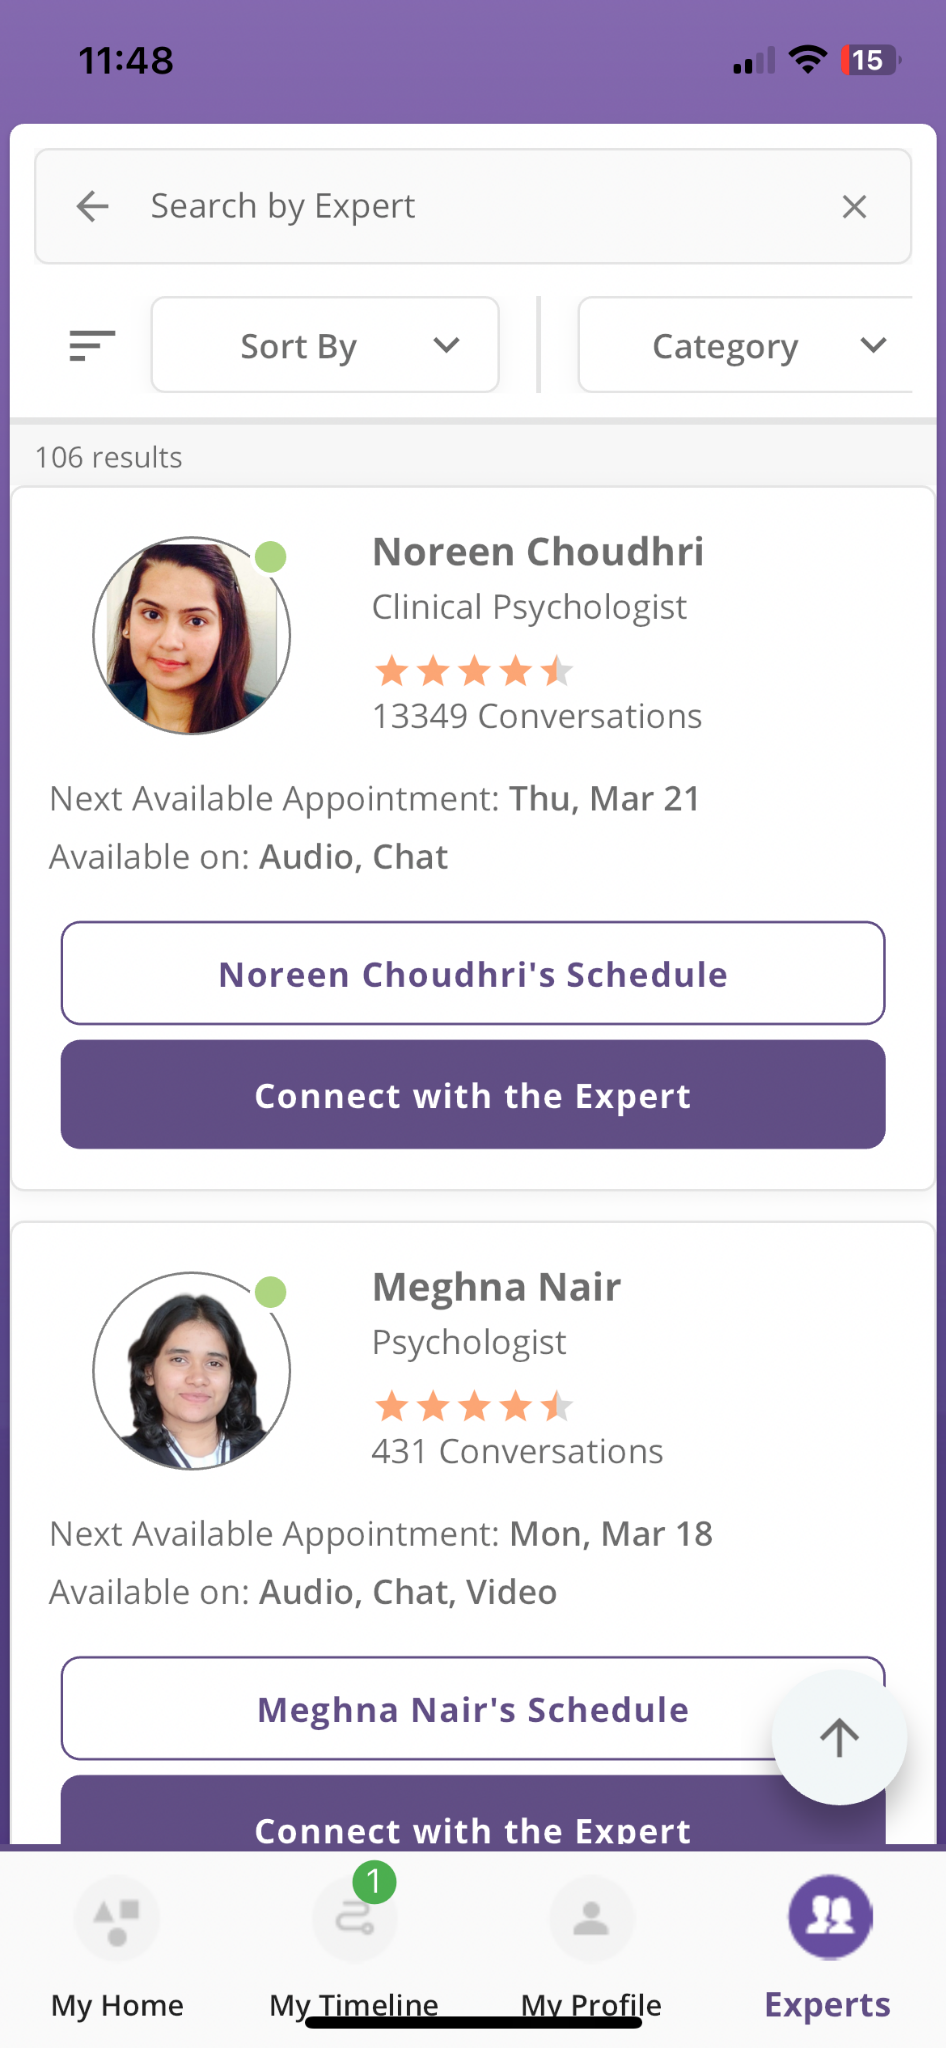
\includegraphics[width=1.49474in,height=3.31321in]{vertopal.com_Untitleddocument/vertopal_25c0ff455f73469eb1b6e3e4452807f6/media/image9.png}
\end{quote}
\begin{enumerate}
\def\labelenumi{\arabic{enumi}.}
\setcounter{enumi}{1}
\item
  \begin{quote}
  Connect with people in similar situations on discussion forums.\\
  \strut \\
  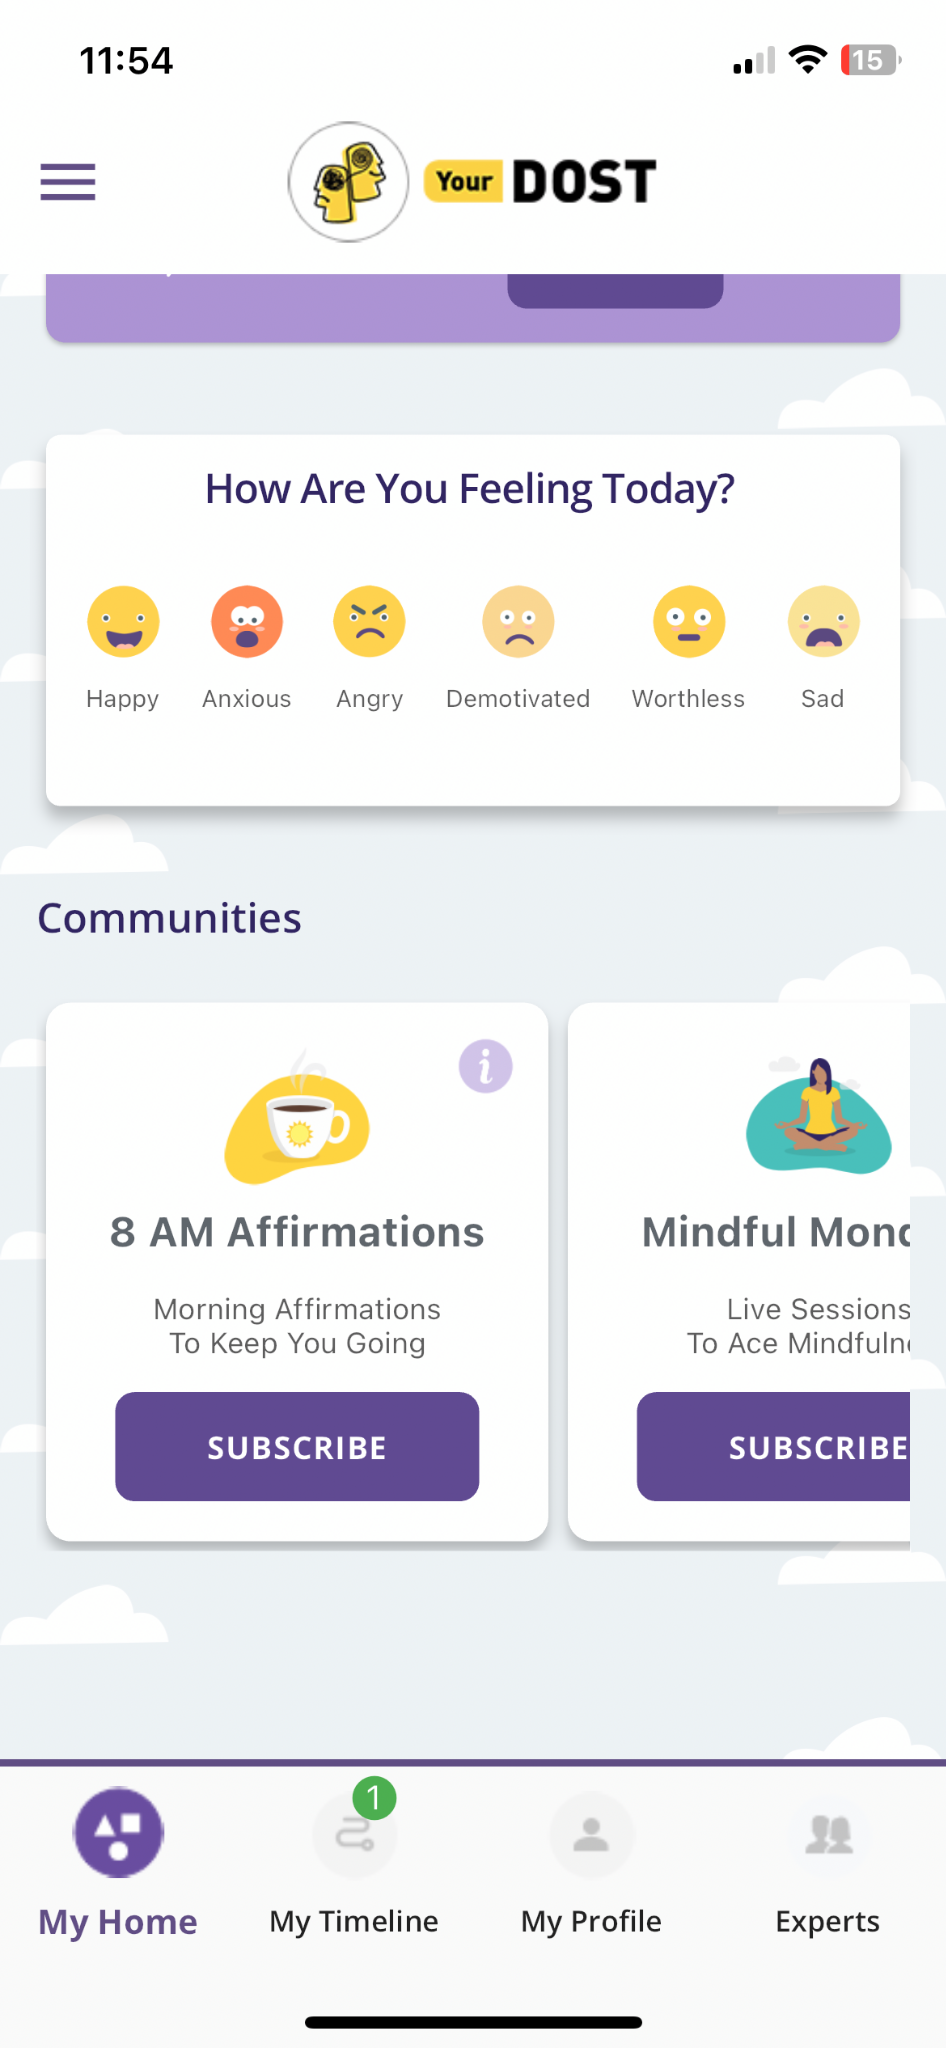
\includegraphics[width=1.49474in,height=3.31321in]{vertopal.com_Untitleddocument/vertopal_25c0ff455f73469eb1b6e3e4452807f6/media/image3.png}
  \end{quote}
\end{enumerate}

\begin{enumerate}
\def\labelenumi{\arabic{enumi}.}
\setcounter{enumi}{2}
\item
  \begin{quote}
  Explore and learn from the wide collection of stories, graphics and
  videos.\\
  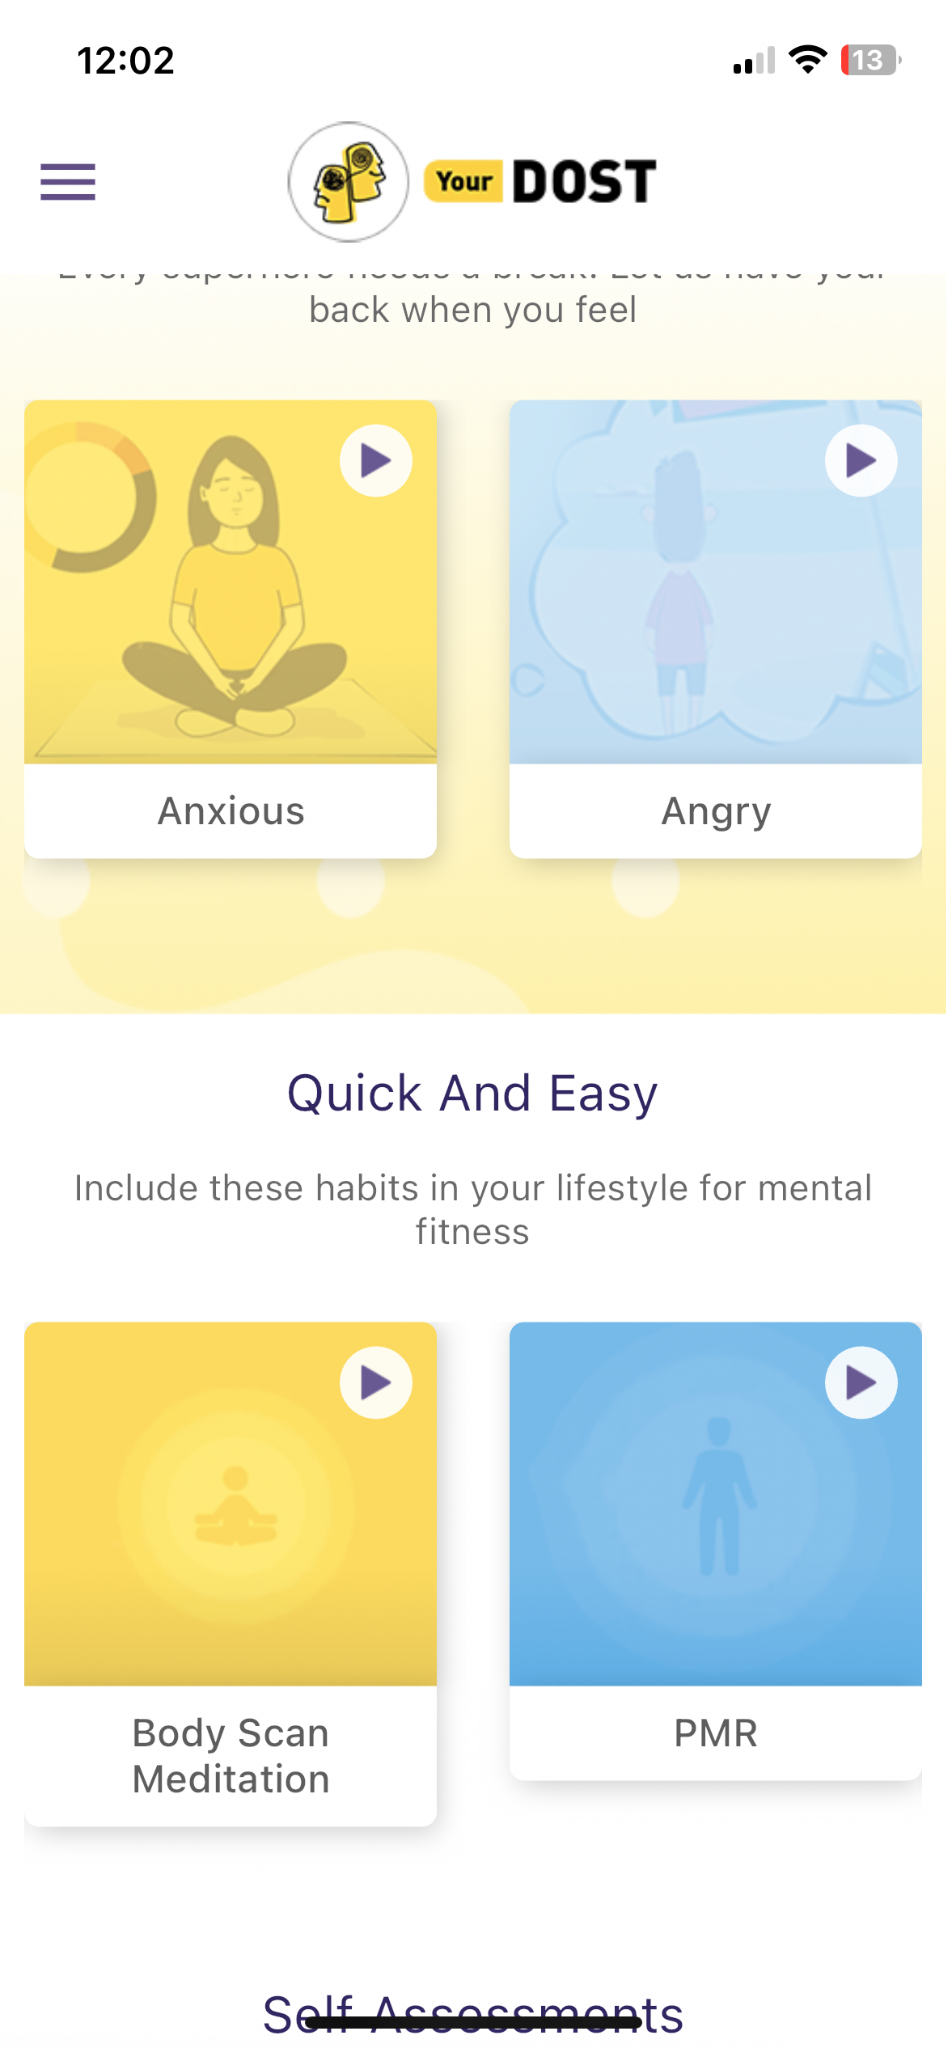
\includegraphics[width=1.49474in,height=3.31321in]{vertopal.com_Untitleddocument/vertopal_25c0ff455f73469eb1b6e3e4452807f6/media/image7.png}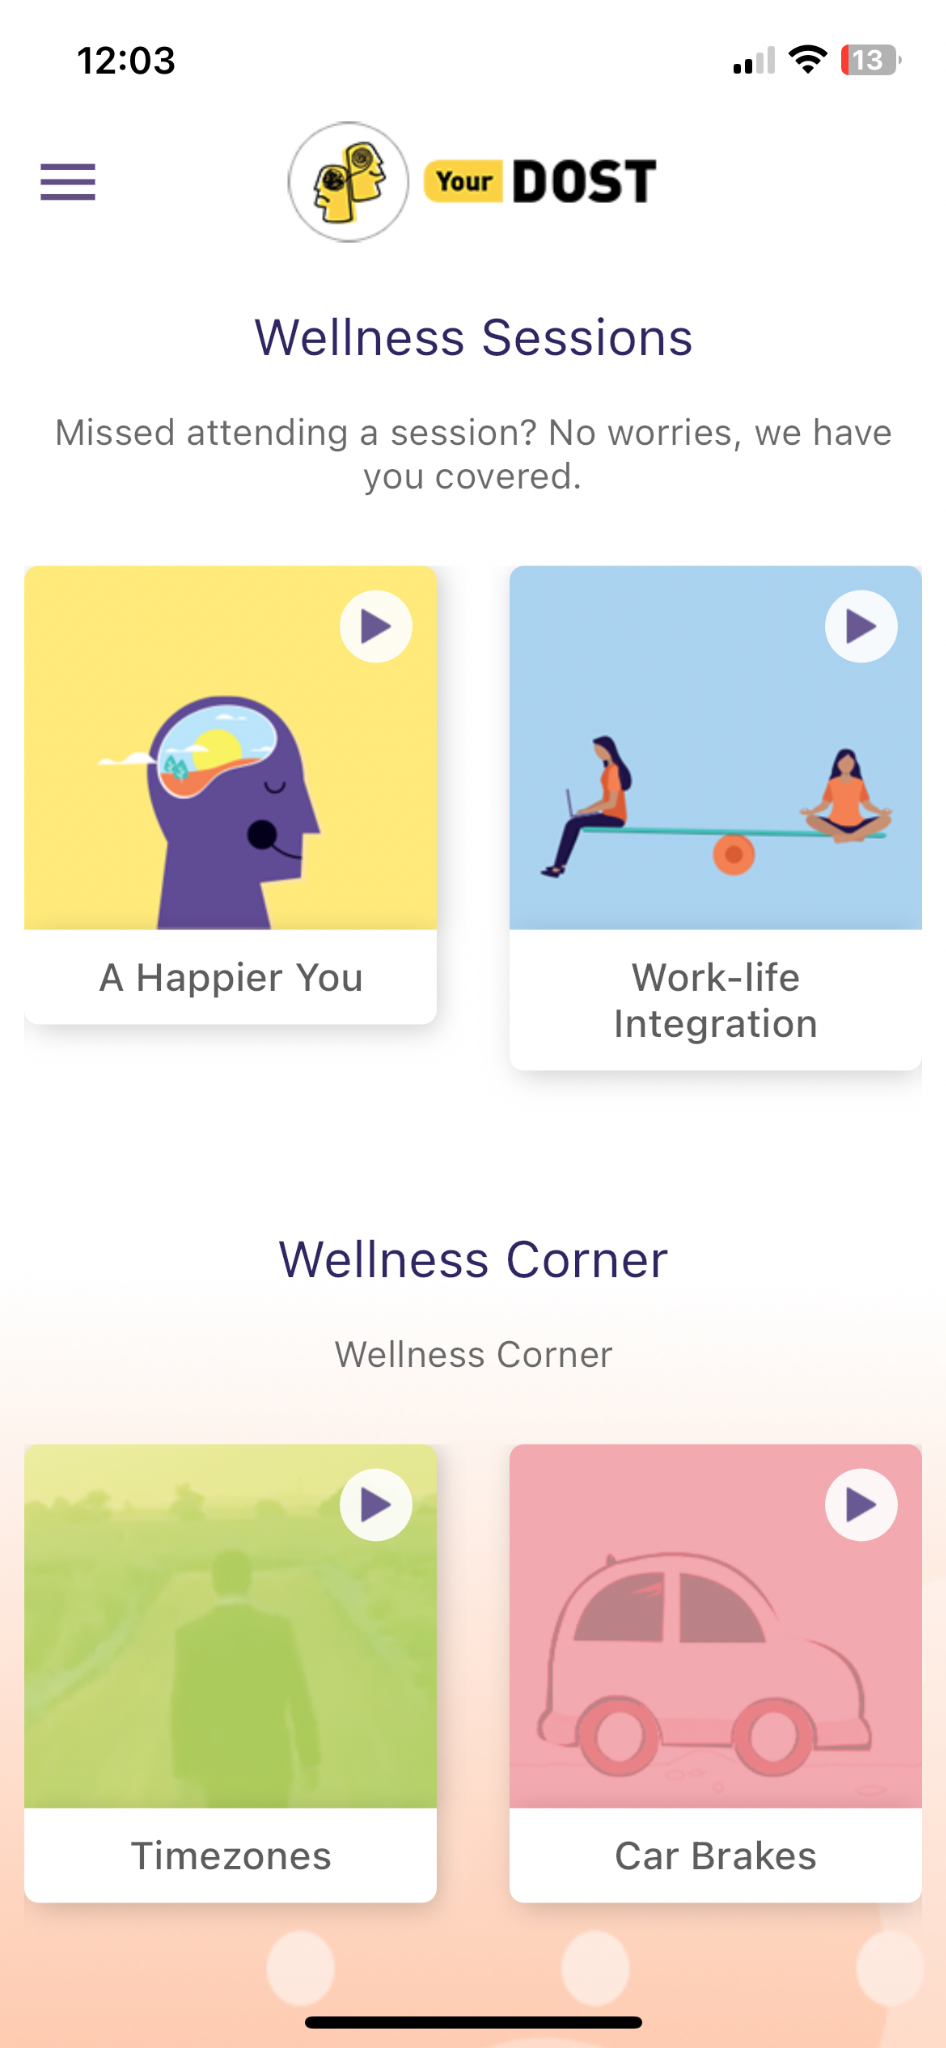
\includegraphics[width=1.65104in,height=3.55846in]{vertopal.com_Untitleddocument/vertopal_25c0ff455f73469eb1b6e3e4452807f6/media/image8.png}\\
  The app offers multiple resources like stories, videos and blogs to
  help users overcome their issues.
  \end{quote}
\item
  \begin{quote}
  Interactive Tests to evaluate user's mental health.\\
  \strut \\
  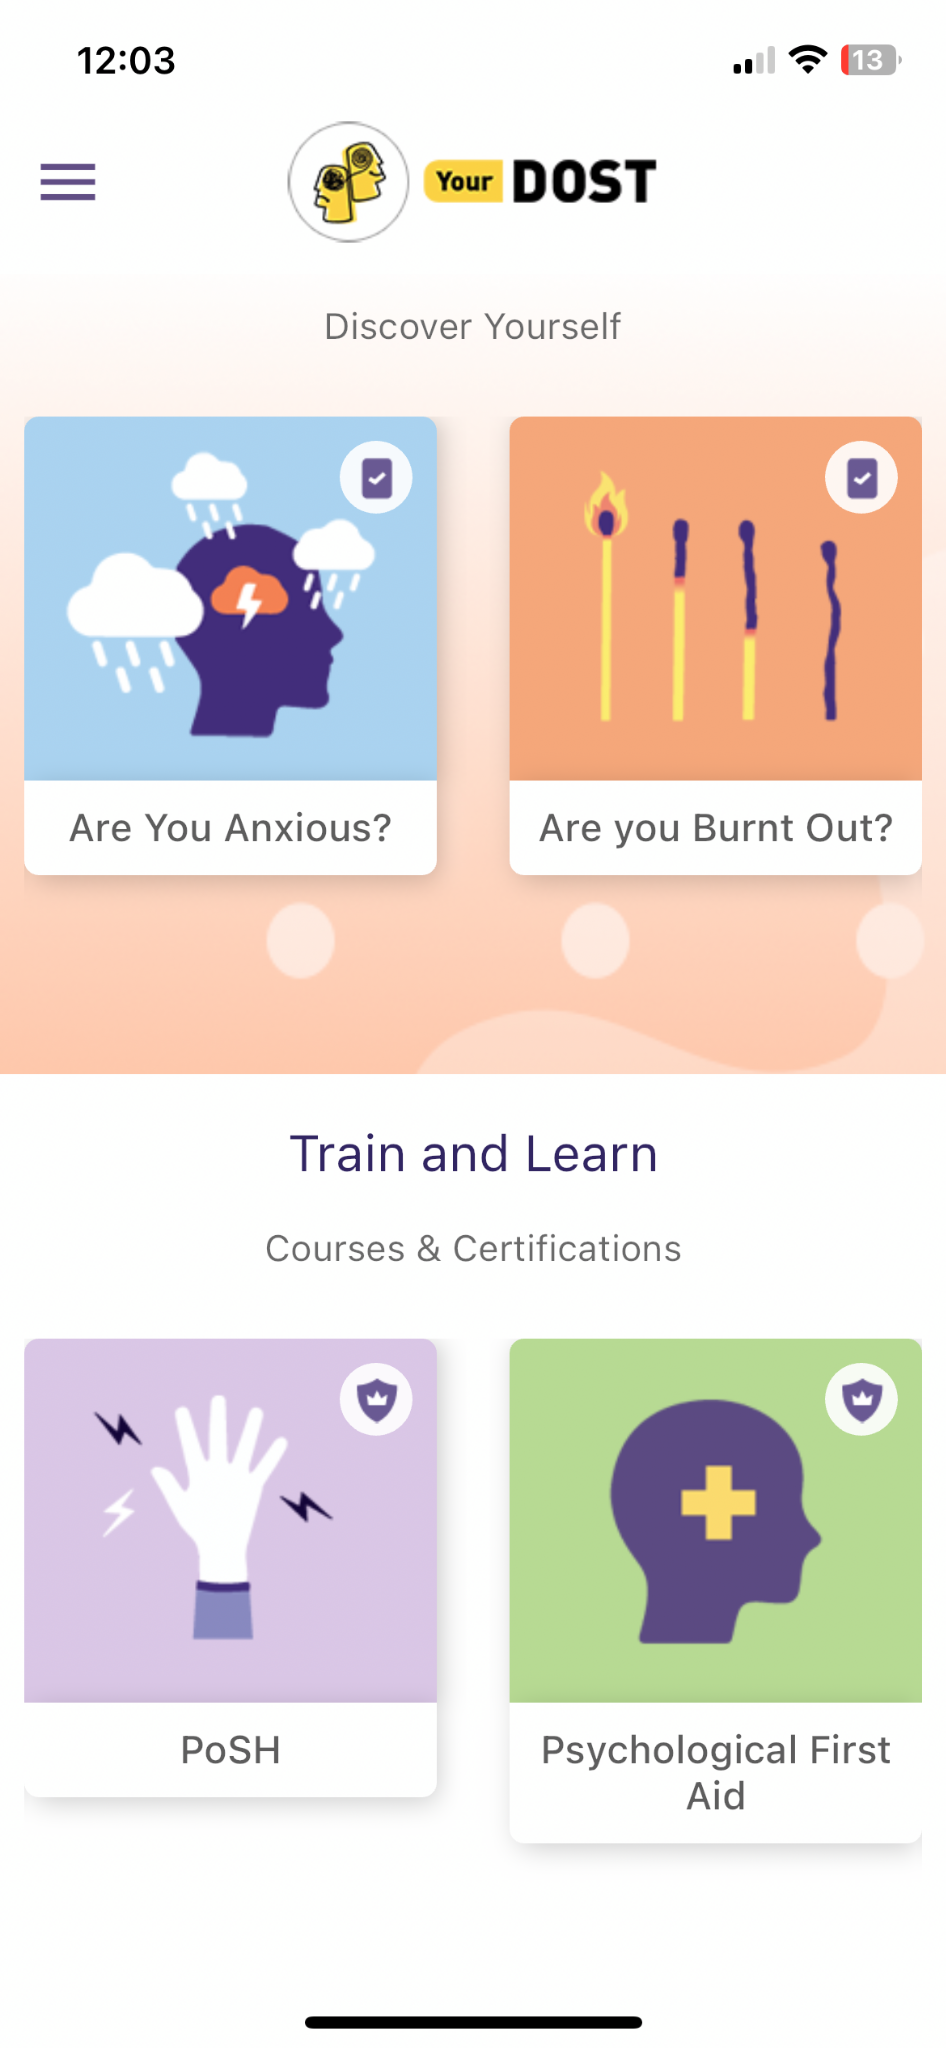
\includegraphics[width=1.49474in,height=3.31321in]{vertopal.com_Untitleddocument/vertopal_25c0ff455f73469eb1b6e3e4452807f6/media/image10.png}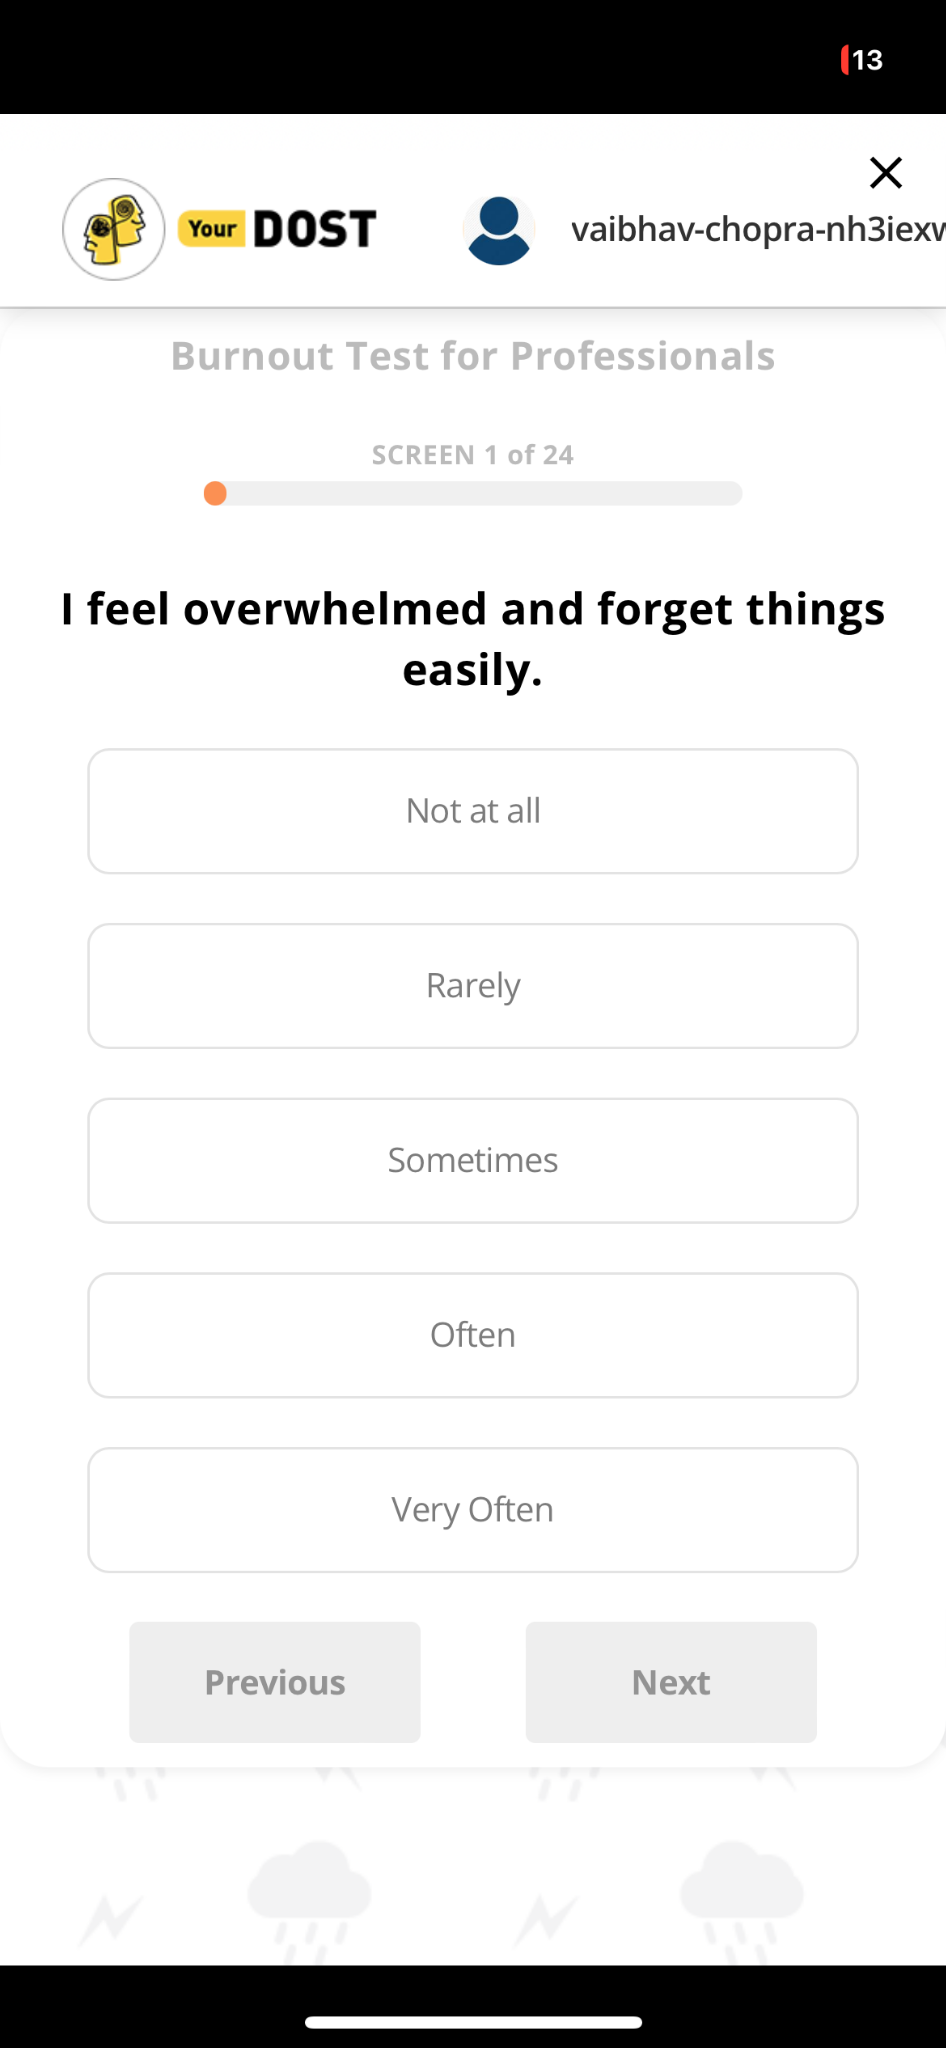
\includegraphics[width=1.49474in,height=3.31321in]{vertopal.com_Untitleddocument/vertopal_25c0ff455f73469eb1b6e3e4452807f6/media/image5.png}
  \end{quote}
\end{enumerate}

\textbf{Product Comparison:}

\begin{itemize}
\item
  \begin{quote}
  \textbf{Gamification Interaction:} The YourDOST app is only integrated
  with a few interactive features like tests and therapy sessions.Our
  app is bundled with various features-\\
  - Daily Challenges: Daily challenges or quests related to mental
  health goals such as practicing mindfulness, journaling, or engaging
  in physical activity.\\
  - Progress Tracking: Visual progress tracking features that allow
  users to monitor their mental health goals over time.\\
  - Interactive Stories: Stories or scenarios within the app that
  simulate real-life situations related to mental health challenges.
  Users can make choices and navigate through the story, with outcomes
  influenced by their decisions.\\
  - Avatar Customization: Users can create and customize their own
  avatars within the app. Users can earn virtual currency or items by
  completing tasks or reaching milestones, which they can use to
  personalize their avatars. This adds a fun and interactive element to
  the app experience.\\
  - Mindfulness Mini-Games: Mini-games or activities focused on
  promoting mindfulness and relaxation techniques such as deep
  breathing, guided meditation, or progressive muscle relaxation. These
  mini-games can serve as quick stress-relief tools that users can
  access whenever they need a break.
  \end{quote}
\item
  \begin{quote}
  \textbf{Therapy Services:} Both the apps provide offline and online
  therapy sessions with experts with a personal chat or a video call.
  \end{quote}
\item
  \begin{quote}
  \textbf{Pricing Strategy:} Both the apps are completely free to use
  for their online services, and are paid for the offline therapy
  sessions.
  \end{quote}
\end{itemize}

\textbf{2. Wysa}

\href{https://www.wysa.com/}{\uline{Wysa}} is an AI-powered mental
health app designed to provide users with emotional support, self-help
tools, and therapeutic techniques to improve their well-being. With a
variety of tools and techniques rooted in evidence-based therapy, Wysa
provides personalized support to help the user build resilience, manage
emotions, and live a happier, healthier life.

\textbf{Product Features:}
\begin{enumerate}
\def\labelenumi{\arabic{enumi}.}
\item
  \begin{quote}
  Emotional Support: Chat feature with AI Wysa anytime, anywhere, and
  receive empathetic responses and evidence-based techniques to help the
  user navigate life\textquotesingle s challenges.\\
  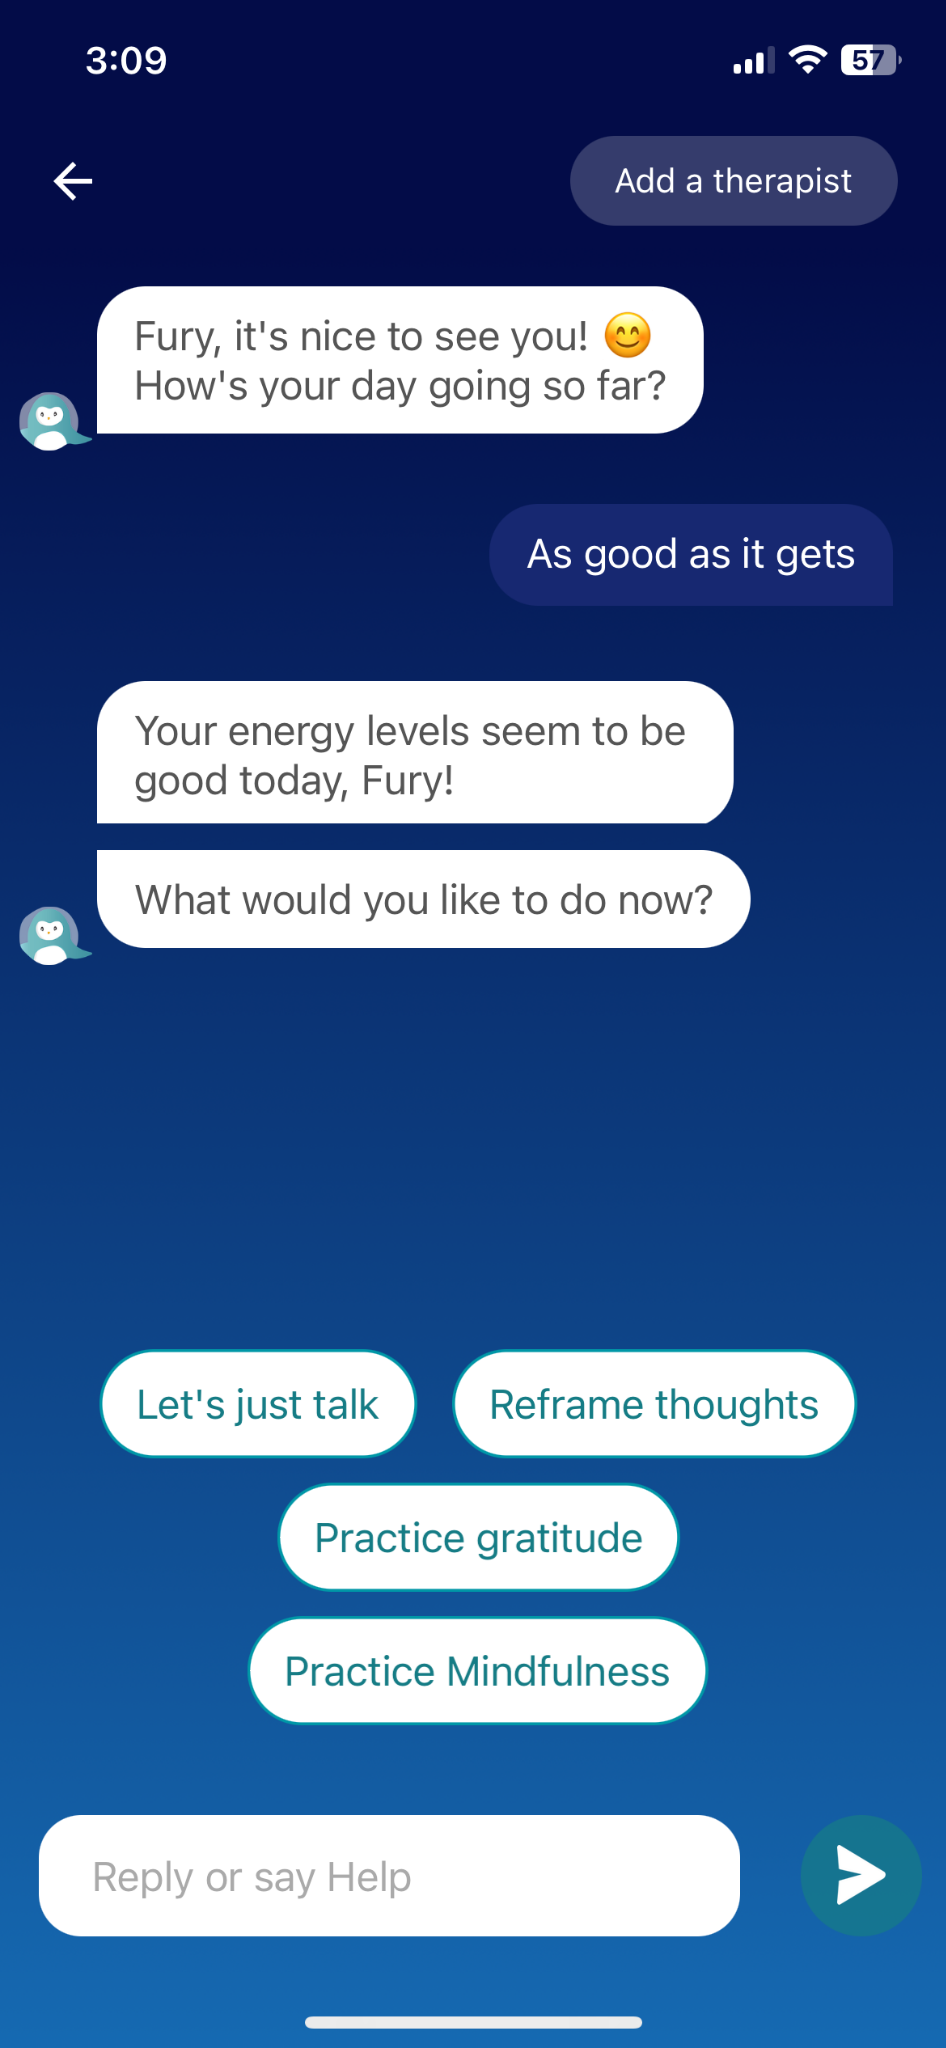
\includegraphics[width=1.49474in,height=3.31321in]{vertopal.com_Untitleddocument/vertopal_25c0ff455f73469eb1b6e3e4452807f6/media/image2.png}
  \end{quote}
\item
  \begin{quote}
  Therapy Sessions with experts: The user can book online therapy
  sessions with highly qualified experts for more personalized
  experience.\\
  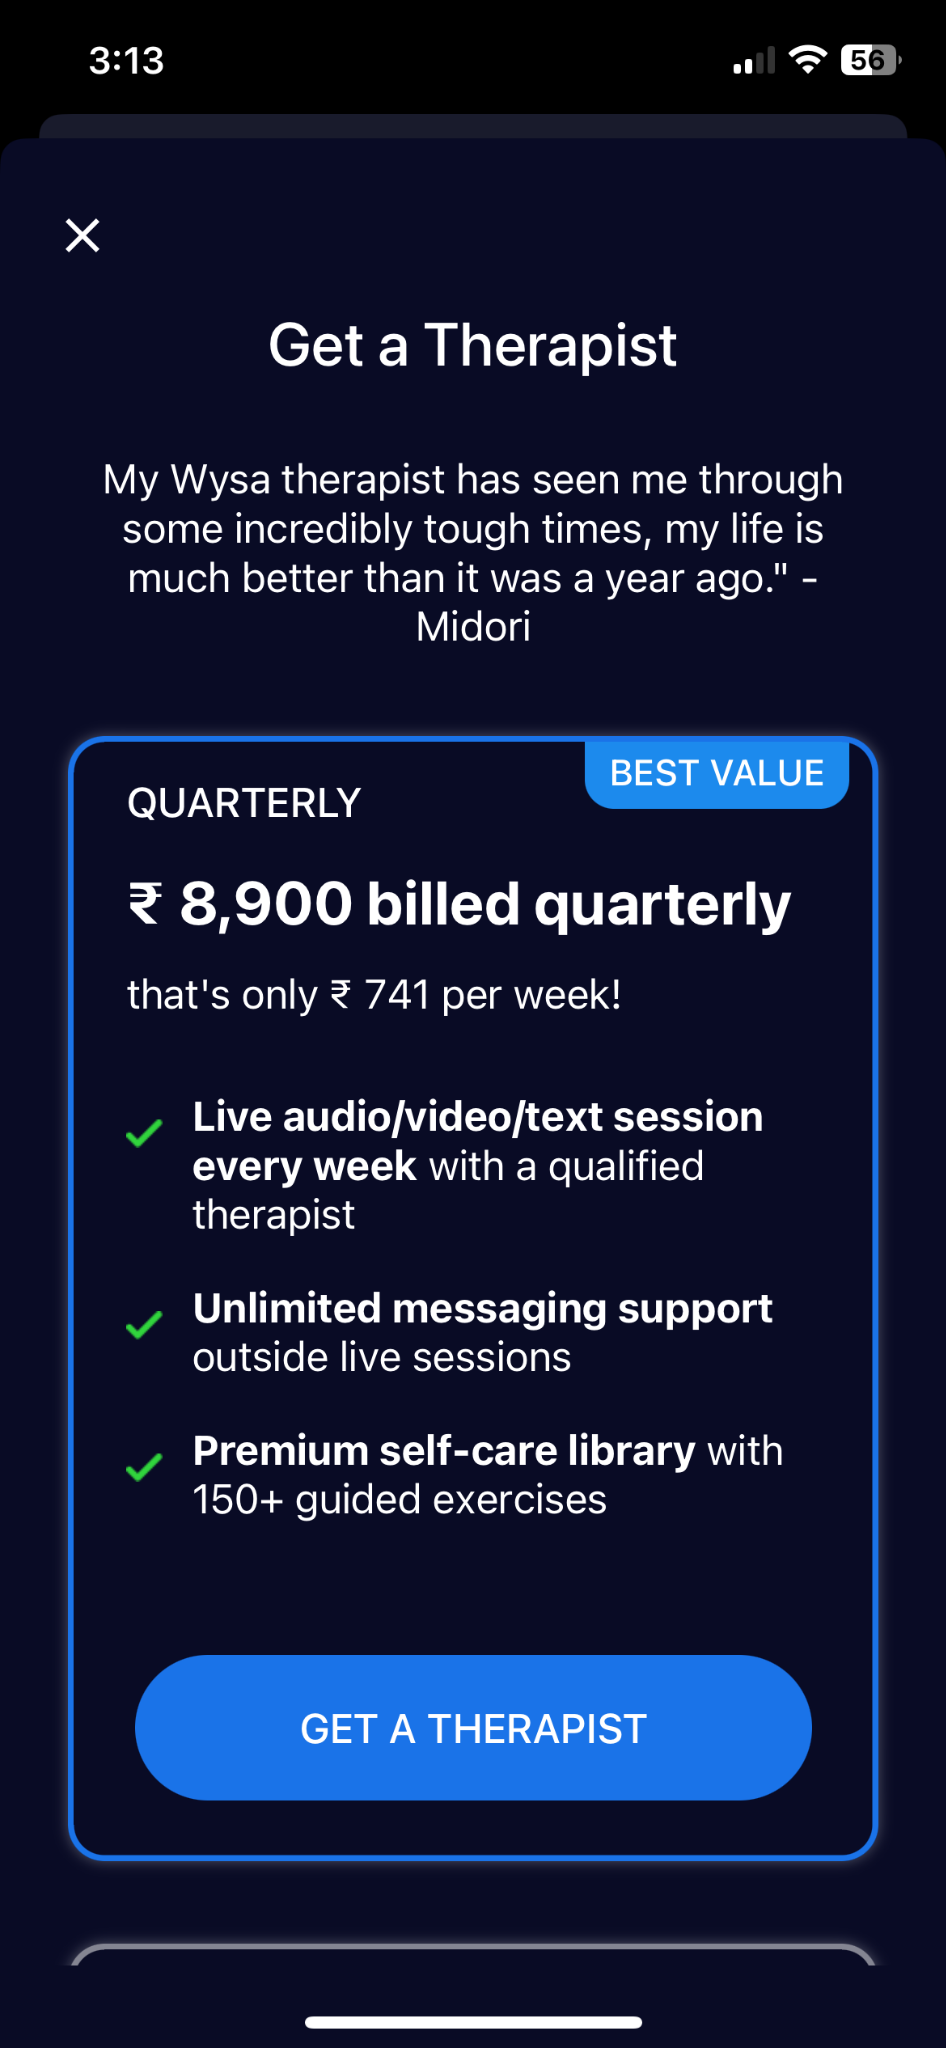
\includegraphics[width=1.49474in,height=3.31321in]{vertopal.com_Untitleddocument/vertopal_25c0ff455f73469eb1b6e3e4452807f6/media/image1.png}
  \end{quote}
\item
  \begin{quote}
  Self-Help Tools: a wide range of self-help exercises and activities,
  including mindfulness meditation, breathing exercises, journaling
  prompts, and mood tracking tools.\\
  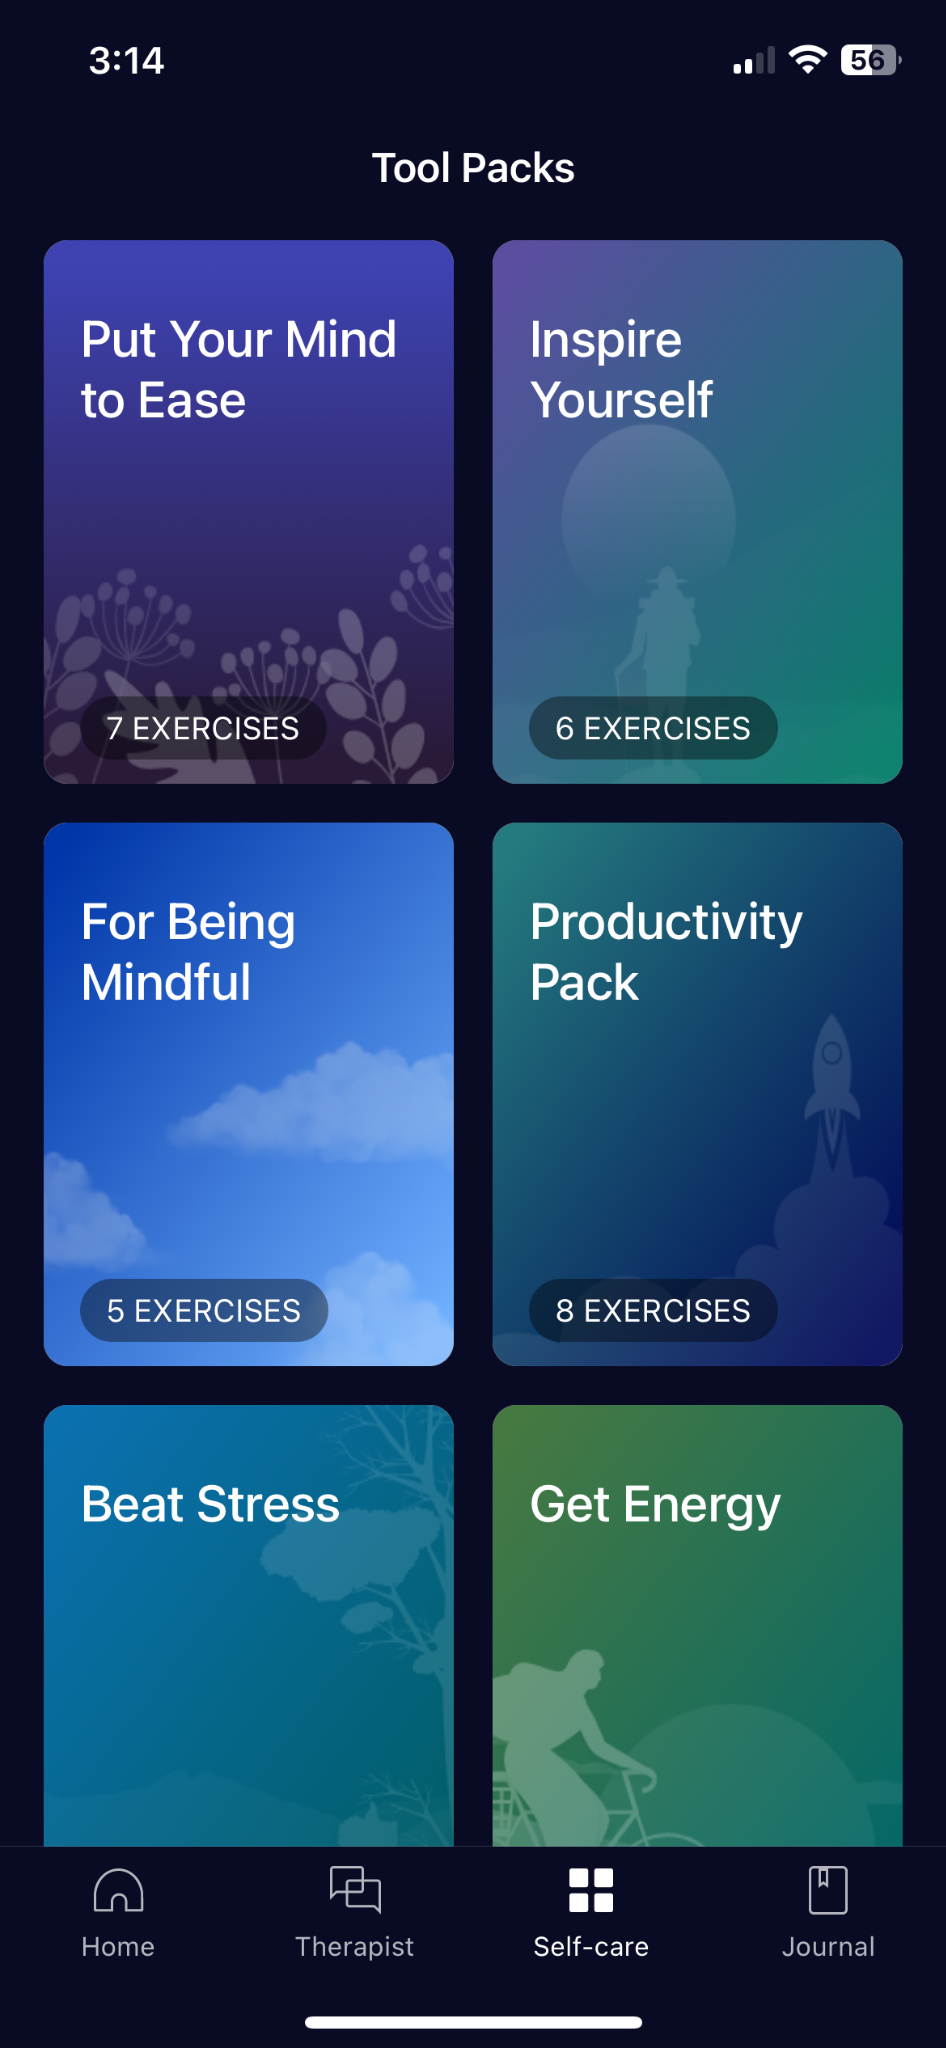
\includegraphics[width=1.49474in,height=3.31321in]{vertopal.com_Untitleddocument/vertopal_25c0ff455f73469eb1b6e3e4452807f6/media/image4.png}
  \end{quote}
\item
  \begin{quote}
  Cognitive Behavioral Therapy (CBT): CBT-based exercises and techniques
  to challenge negative thought patterns, reframe unhelpful beliefs, and
  build healthier coping strategies.\\
  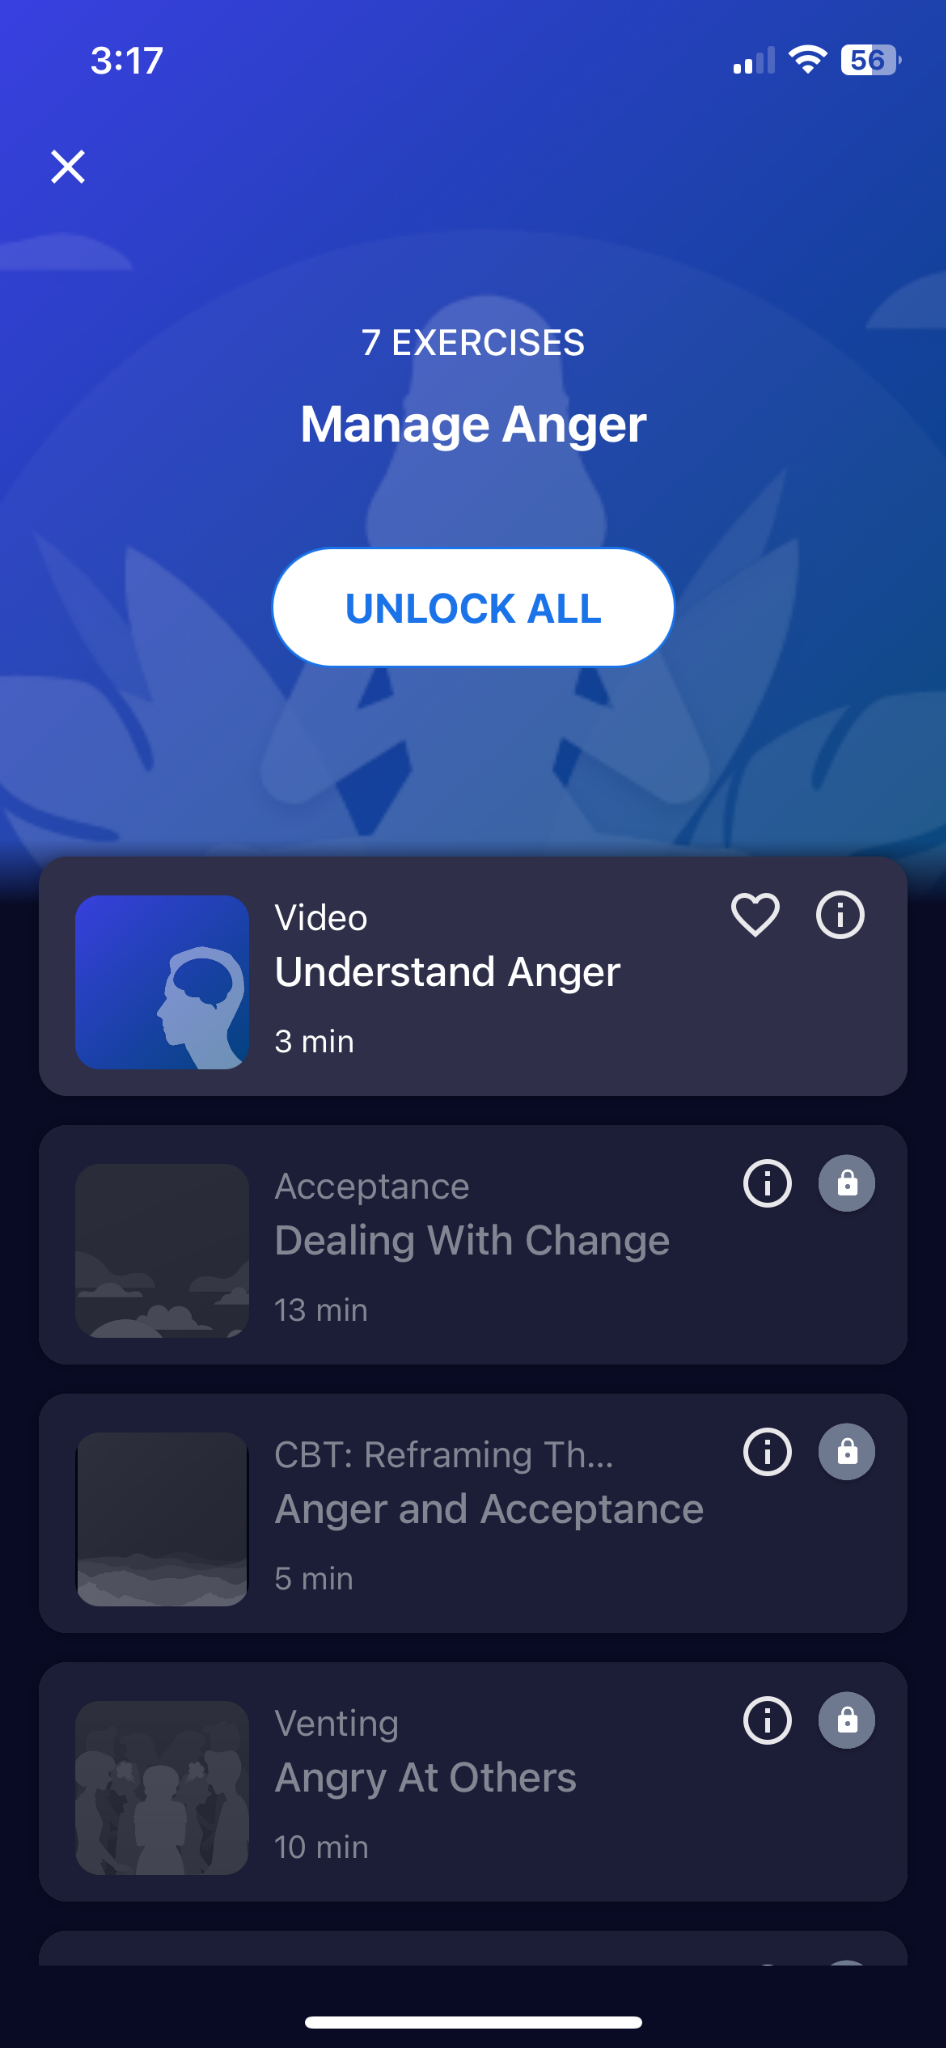
\includegraphics[width=1.49474in,height=3.31321in]{vertopal.com_Untitleddocument/vertopal_25c0ff455f73469eb1b6e3e4452807f6/media/image6.png}
  \end{quote}
\end{enumerate}

\textbf{Product Comparison:}

\begin{itemize}
\item
  \begin{quote}
  \textbf{Gamification Interaction:} The Wysa app has a lot of
  interactive features like the AI chatbot but lacks gamified elements
  that our app provides-\\
  - Daily Challenges: Daily challenges or quests related to mental
  health goals such as practicing mindfulness, journaling, or engaging
  in physical activity.\\
  - Progress Tracking: Visual progress tracking features that allow
  users to monitor their mental health goals over time.\\
  - Interactive Stories: Stories or scenarios within the app that
  simulate real-life situations related to mental health challenges.
  Users can make choices and navigate through the story, with outcomes
  influenced by their decisions.\\
  - Avatar Customization: Users can create and customize their own
  avatars within the app. Users can earn virtual currency or items by
  completing tasks or reaching milestones, which they can use to
  personalize their avatars. This adds a fun and interactive element to
  the app experience.\\
  - Mindfulness Mini-Games: Mini-games or activities focused on
  promoting mindfulness and relaxation techniques such as deep
  breathing, guided meditation, or progressive muscle relaxation. These
  mini-games can serve as quick stress-relief tools that users can
  access whenever they need a break.
  \end{quote}
\item
  \begin{quote}
  \textbf{Therapy Sessions:} The Wysa app only provides online therapy
  sessions with chat/video/text sessions. Our app provides both online
  and offline services
  \end{quote}
\item
  \begin{quote}
  \textbf{Pricing Strategy:} A lot of features of the Wysa app like
  therapy sessions and half of the Self-Help tools are behind a paywall,
  with pricing starting at 10\$ a week. Our app provides all the online
  features free of cost.
  \end{quote}
\end{itemize}

\section{Patents and Concepts Utilised}

Several key concepts and principles are used in the development of a gamified version of a mental health application. We have identified concepts from three main broader areas: User-Centered Design, Gamification and Digital Health and Behavioral Science. 
\\ \\
Robson et al. \cite{Robson15} (2015) point to the importance of incorporating game design elements into non-game contexts to increase user engagement. The application can then leverage motivational drivers such as autonomy, mastery, and purpose while integrating game mechanics like points, badges, and levels to provide feedback and encourage desired behaviors. Personalization based on user preferences and goals should be a central focus, ensuring that gamified elements resonate with individual users.
\\ \\
Conducting thorough user research also becomes paramount, enabling the identification of specific mental health needs, challenges, and preferences. Users should be actively involved through an iterative design process from initial concept development to usability testing. Personalization should extend beyond content to encompass the app's features and gamified elements, ensuring that the application is intuitive, accessible, and relevant to users of diverse backgrounds and abilities \cite{Schnall16}.
\\ \\
Finally, as highlighted by Eysenbach \cite{Eysenbach05} (2005) and Christensen and Mackinnon \cite{Christensen06} (2006), addressing the challenge of attrition requires strategic intervention to sustain user engagement over time. By understanding factors influencing attrition, such as usability issues, perceived lack of benefit, or competing demands, the application can implement strategies to promote continued usage. This includes ongoing monitoring of user engagement metrics and iterative app refinement based on user feedback and usage data. 
\\ \\
By integrating these principles into the development process, the gamified mental health application can effectively support users' mental well-being while fostering sustained engagement and positive outcomes.




\section{Requirement Gathering}

\subsection{User Requirements}
\begin{enumerate}
    \item \textbf{Engagement and Interactivity:} Users require an interface that maximizes the fun factor in an app without compromising its functionality.
    \item \textbf{Personalization:} Users prefer apps that cater to their preferences and provide personalized suggestions relevant to their needs.
    \item \textbf{Ease of Use:} Users value an interface that is easy to use, as it enhances their overall experience.
    \item \textbf{Wide Range of Features:} Users expect apps to offer a variety of features to cater to a diverse user base.
\end{enumerate}

\subsection{Functional Requirements}
\begin{enumerate}
    \item \textbf{Daily Challenges (Gamified):} Incorporate daily quests related to mental health goals, such as mindfulness, journaling, and physical activity.
    \item \textbf{Mood Tracking/Progress Tracking:} Provide functionality for users to monitor their mood over time and track progress with mental health goals.
    \item \textbf{Interactive Stories:} Include story-based scenarios within the app that simulate real-life situations related to mental health challenges.
    \item \textbf{Custom Avatars and Virtual Currency:} Allow users to select custom avatars and earn virtual currency for completing goals.
    \item \textbf{Personalized Recommendations:} Implement algorithms to provide personalized recommendations based on user interactions, preferences, and goals.
\end{enumerate}

\subsection{Environmental Requirements}
\begin{enumerate}
    \item \textbf{Cross-Platform Compatibility:} Ensure the app is accessible across various platforms (iOS, Android, web) to accommodate all users.
    \item \textbf{Privacy and Security:} Implement privacy measures and data encryption to protect user data and comply with regulations such as GDPR and HIPAA.
\end{enumerate}

\subsection{Usability Requirements}
\begin{enumerate}
    \item \textbf{Intuitive User Interface (UI):} Design an easy-to-use interface with clear instructions and minimal ambiguity about navigation.
    \item \textbf{Accessibility Features:} Incorporate basic accessibility principles to address potential usability issues for users with disabilities.
    \item \textbf{Onboarding Process:} Use graphics and animations to facilitate the onboarding process and help users quickly grasp app concepts.
    \item \textbf{Customization Options:} Provide users with customization options to enhance usability and make them feel more in control of the app.
\end{enumerate}



\section{Personas}

    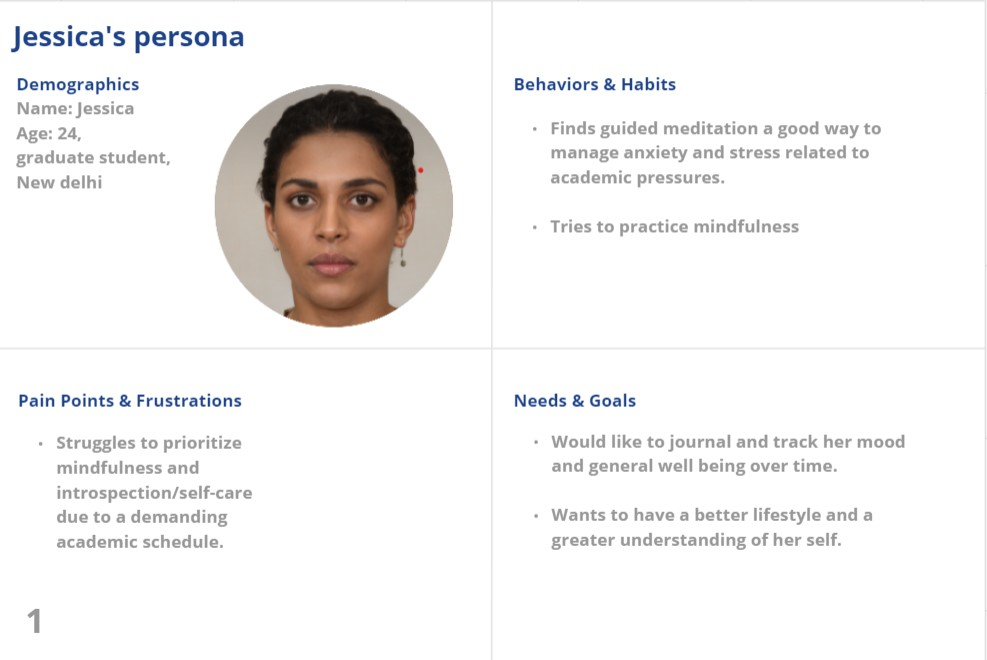
\includegraphics[width=6.26806in,height=4.19375in]{vertopal.com_Personas/vertopal_68c5e293405b4e92b3a0f3d4afe53fc3/media/image1.jpeg}


    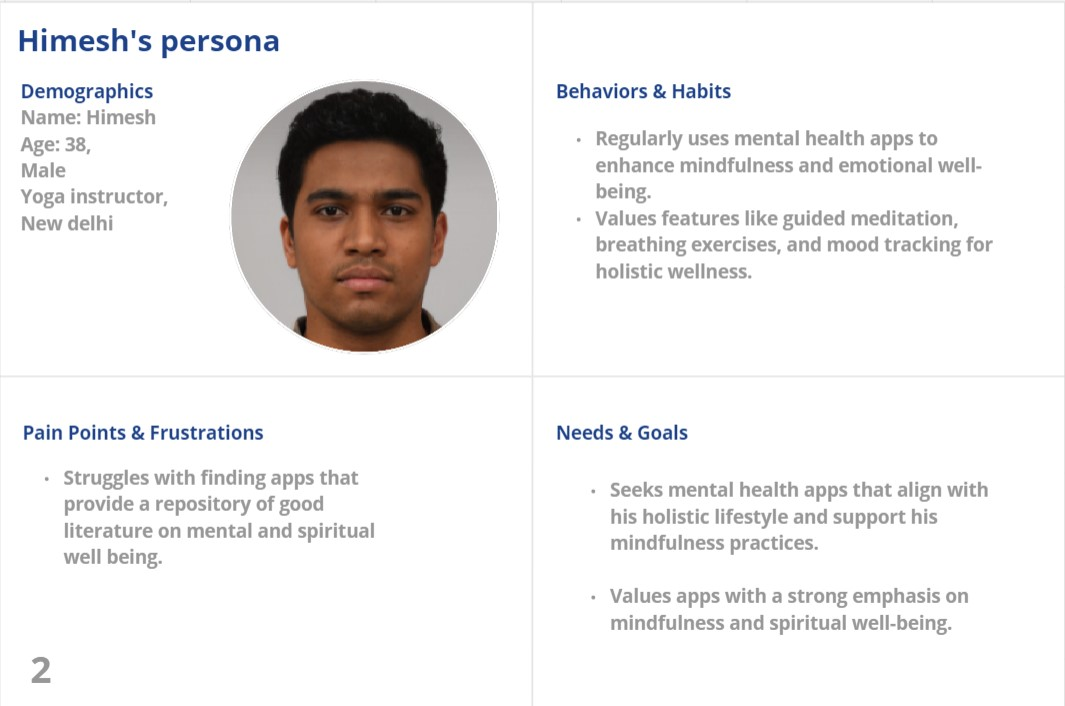
\includegraphics[width=6.26806in,height=4.15764in]{vertopal.com_Personas/vertopal_68c5e293405b4e92b3a0f3d4afe53fc3/media/image2.jpeg}



    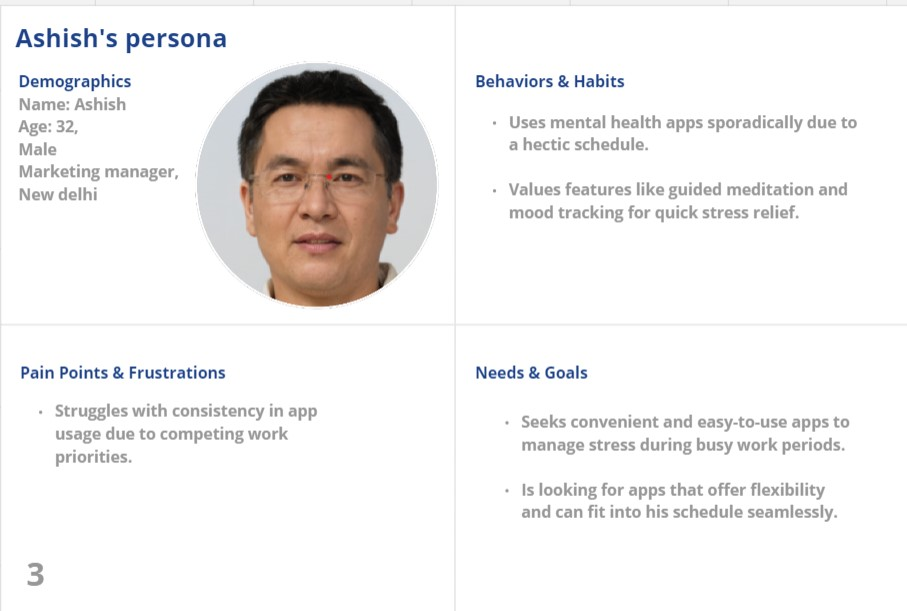
\includegraphics[width=6.26806in,height=4.22222in]{vertopal.com_Personas/vertopal_68c5e293405b4e92b3a0f3d4afe53fc3/media/image3.jpeg}

    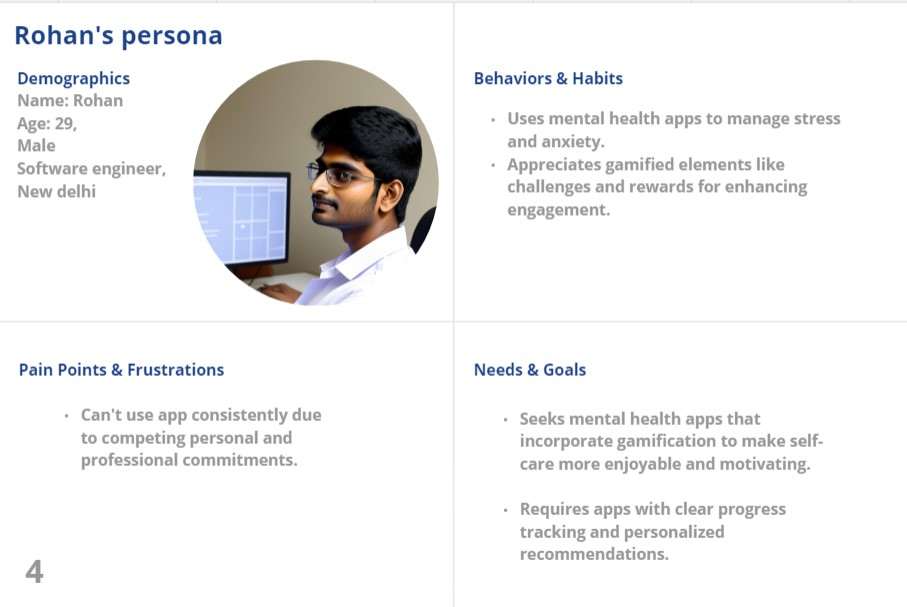
\includegraphics[width=6.26806in,height=4.19722in]{vertopal.com_Personas/vertopal_68c5e293405b4e92b3a0f3d4afe53fc3/media/image4.jpeg}


\newline


\section{Interview Analysis (Qualitative)}
Click \href{https://docs.google.com/document/d/1MPaA-0VwmMxalHK1cTz1QMZmGF4sPHEAJa-ONISMrXk/edit}{here} to access the transcript.

\begin{enumerate}
    \item \textbf{Experience with Mental Health Apps:}
    \begin{itemize}
        \item Most participants are aware of meditation and mindfulness apps, not mental health apps per se.
        \item People are generally very inconsistent in their usage of such apps. This discovery further fuels our conception that these apps lack user retention and engagement.
    \end{itemize}
    
    \item \textbf{Mental Health and Gamification:}
    \begin{itemize}
        \item An understanding of what mental health and gamification mean to people.
        \item People relate mental health with emotional, psychological and social well-being.
        \item Participants described gamification as incorporating game-like elements into apps and other technologies with different contexts.
    \end{itemize}
    
    \item \textbf{Perception of Gamification in Mental Health Apps:}
    \begin{itemize}
        \item There is a unanimous agreement that gamification would make mental health apps more effective and fun to use.
        \item Most participants believe gamification has the potential to make these apps more interactive and convivial.
        \item Features such as challenges, rewards, progress tracking, animated interfaces, and leaderboards lead to piqued user interest.
    \end{itemize}
    
    \item \textbf{Preferences and Needs:}
    \begin{itemize}
        \item Personalization of any technology makes it more desirable.
        \item One participant highlighted that looking for good therapists near him is painstaking.
        \item Social features like online support groups might be a good addon.
    \end{itemize}
    
    \item \textbf{Frustrations:}
    \begin{itemize}
        \item Lack of consistently reliable information sources on mental health issues.
        \item Online solutions or platforms for dealing with mental health issues are often drab and not fun to use.
        \item The perceived utility of such apps is also poor.
    \end{itemize}
    
    \item \textbf{Concerns and Suggestions:}
    \begin{itemize}
        \item One big concern is that gamification might overshadow actual therapy-related content.
        \item Looking at stress, anxiety, and depression as parts of the same bracket might not be a good idea.
    \end{itemize}
\end{enumerate}
\newline
\textbf{Overall Analysis:} The analysis highlights users' perceptions of mental health apps. Generally speaking, people are neutral about using them (from what our survey data tells us). They have concerns about the effectiveness and concreteness of such solutions to mental health issues. Gamification is perceived positively, and people immediately relate to the concept and find it useful for enhancing engagement. The balance between gamification and the content of actual substance is another concern that users have. Additionally, users' preferences for personalized features emphasize the need for customization options to cater to diverse user needs and preferences.




\section{Survey Analysis}

Demographic questions relevant to our study:

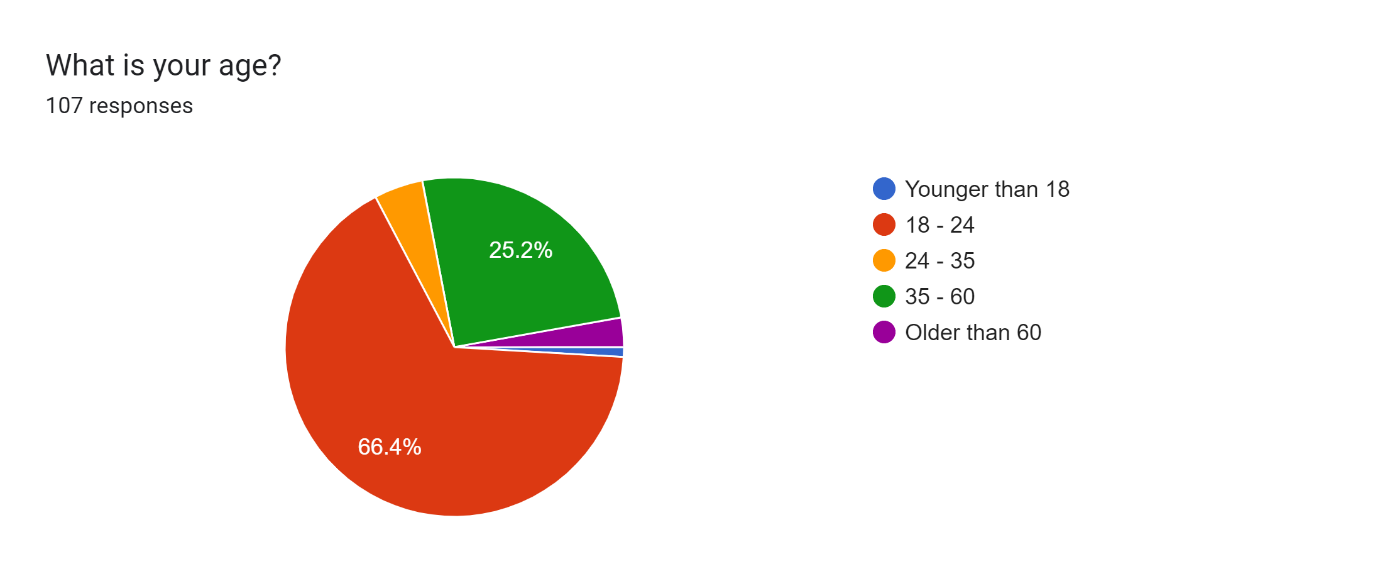
\includegraphics[width=6.26806in,height=2.63889in]{vertopal.com_Survey analysis/vertopal_0d4ab446a1ae41f4824d7f0aaede9ca1/media/image1.png}

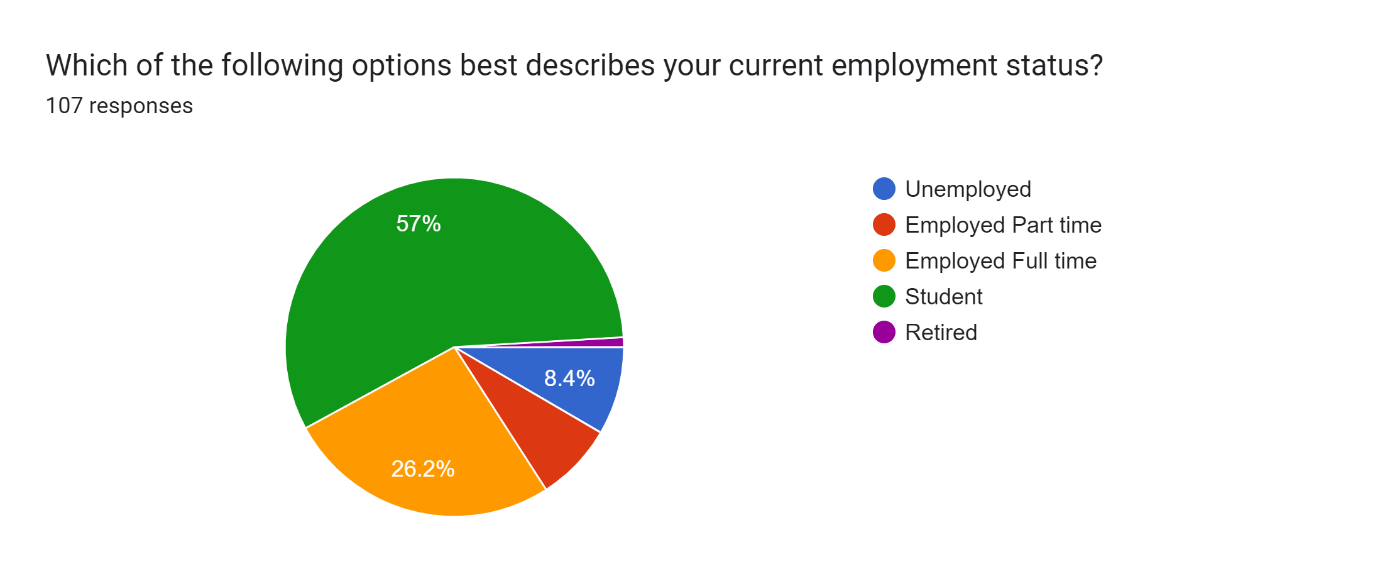
\includegraphics[width=6.26806in,height=2.63889in]{vertopal.com_Survey analysis/vertopal_0d4ab446a1ae41f4824d7f0aaede9ca1/media/image2.png}

We interviewed a good mix of people from different sections of the job
spectrum and age groups to paint a comprehensive picture. The sample may
be slightly biased, with the most responses coming in from students aged
18-24 because it is the most accessible section for us. Despite the
bias, the picture might not be skewed because the user base of such apps
includes a similar proportion of a young population, as shown below:

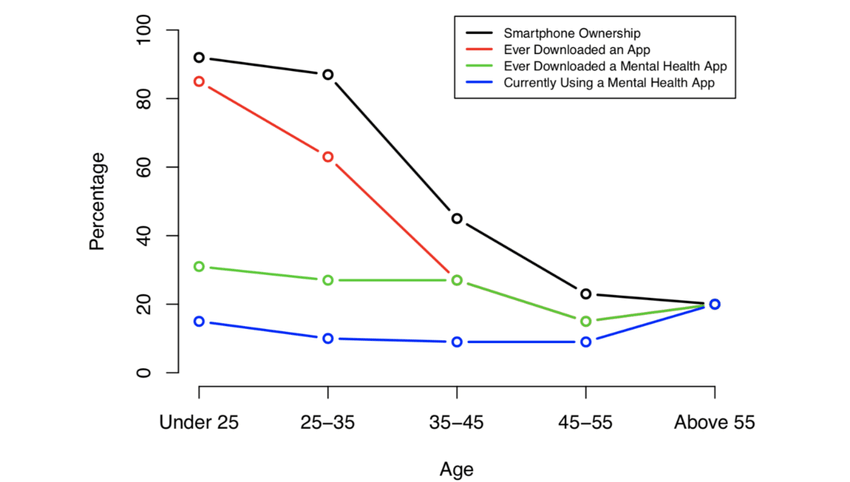
\includegraphics[width=3.74872in,height=2.12522in]{vertopal.com_Survey analysis/vertopal_0d4ab446a1ae41f4824d7f0aaede9ca1/media/image3.png}

Source:
\href{https://www.researchgate.net/figure/Mobile-phone-ownership-app-downloads-mental-health-app-downloads-and-mental-health-app_fig2_328373517}{link}

The graph above shows how smartphone ownership and mental health app
downloads decrease with age

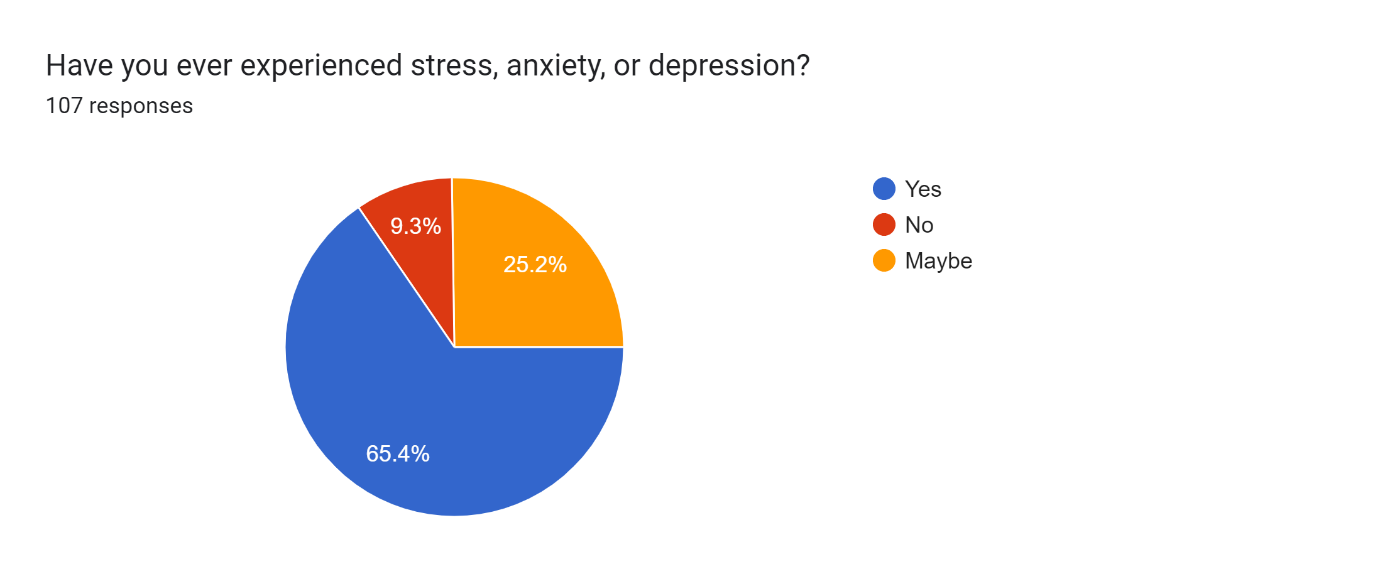
\includegraphics[width=6.26806in,height=2.63889in]{vertopal.com_Survey analysis/vertopal_0d4ab446a1ae41f4824d7f0aaede9ca1/media/image4.png}

This mapping of the responses is self-explanatory. Most people who took
our survey (65.4\%, to be precise) have experienced stress, anxiety, or
depression in their lifetime.

The interesting section here is the 25.2\% of people who responded with
``maybe.'' A staggering proportion of people do not know if they had
such issues in the past. Our app aims to help such people identify with
the common issues other people have faced or are still facing.

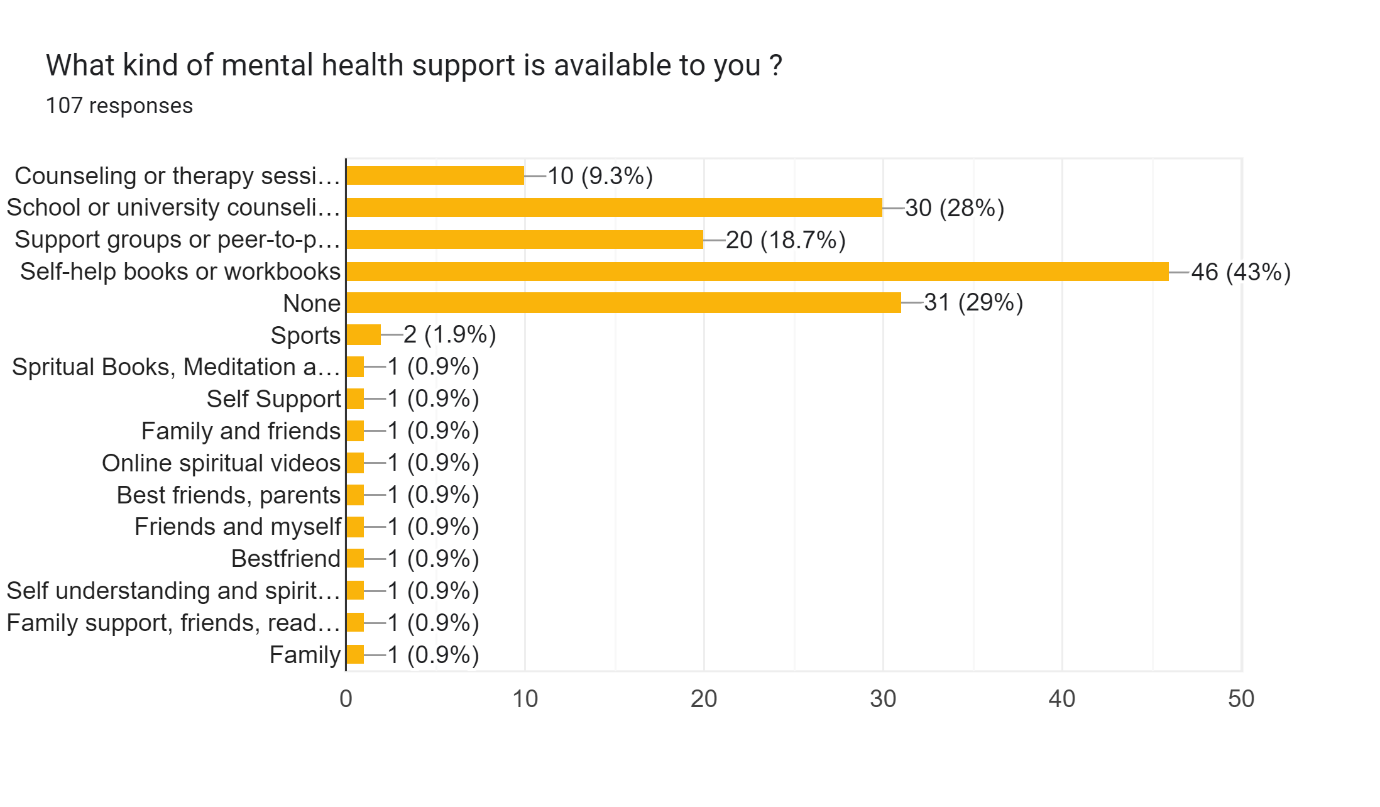
\includegraphics[width=6.26806in,height=3.66458in]{vertopal.com_Survey analysis/vertopal_0d4ab446a1ae41f4824d7f0aaede9ca1/media/image5.png}

Here, 31 respondents admitted to having no mental health support system
at all. An app might reduce the friction between these people and some
kind of help. Self-help books or workbooks are the most common resources
used in this regard. We aim to provide a curated collection of
literature on mental health and aid users in finding better resources.

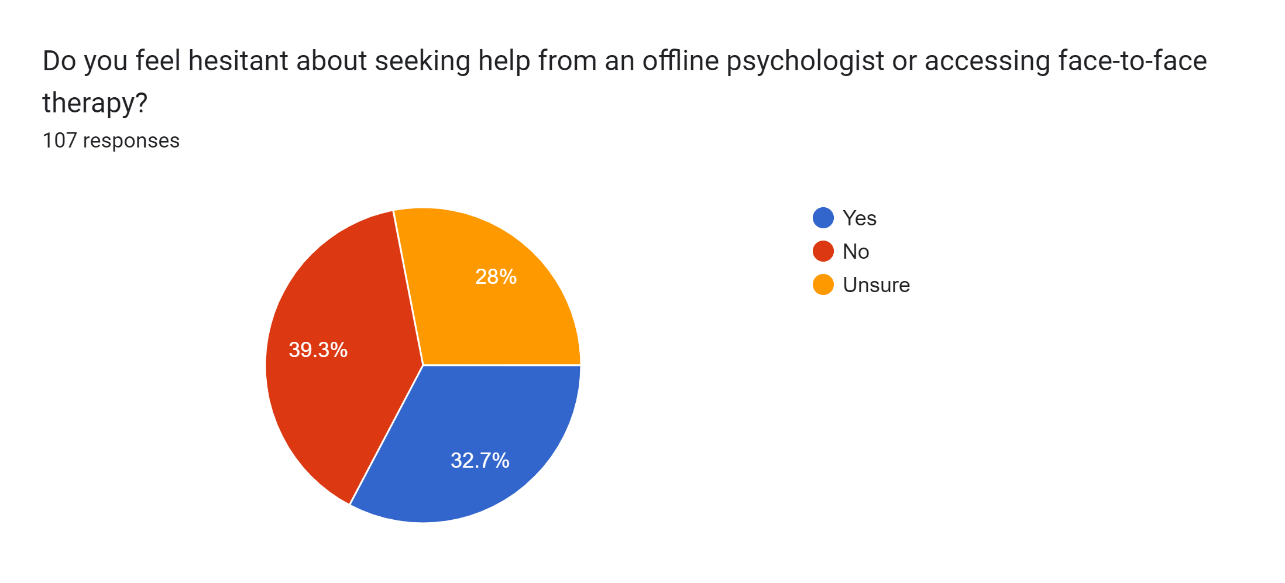
\includegraphics[width=5.84259in,height=2.64943in]{vertopal.com_Survey analysis/vertopal_0d4ab446a1ae41f4824d7f0aaede9ca1/media/image6.png}

This question delves deeper into the reasons why people do not have
robust support systems. One of the biggest reasons is hesitance (also
misinformation). As mentioned earlier, an app might make it easier for
people to consult, say, a therapist over the internet for minor mental
health issues (some of which they may not even be aware of). The app
would also recommend well-reputed psychiatrists nearby for offline
consultation.

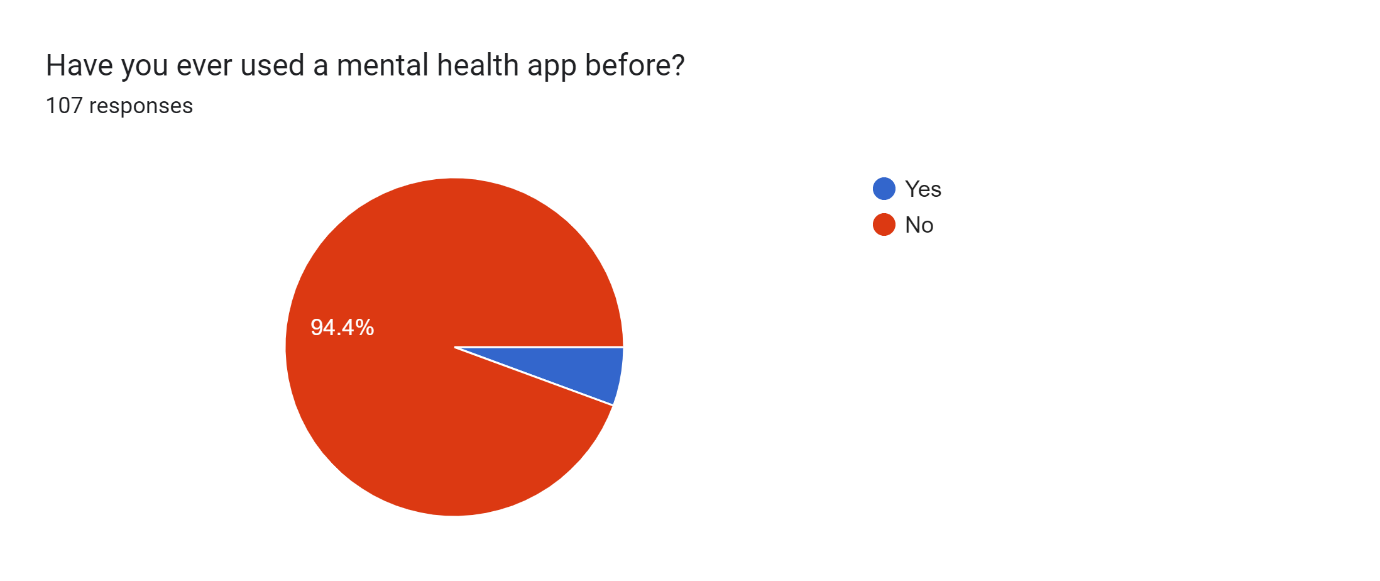
\includegraphics[width=6.26806in,height=2.63889in]{vertopal.com_Survey analysis/vertopal_0d4ab446a1ae41f4824d7f0aaede9ca1/media/image7.png}

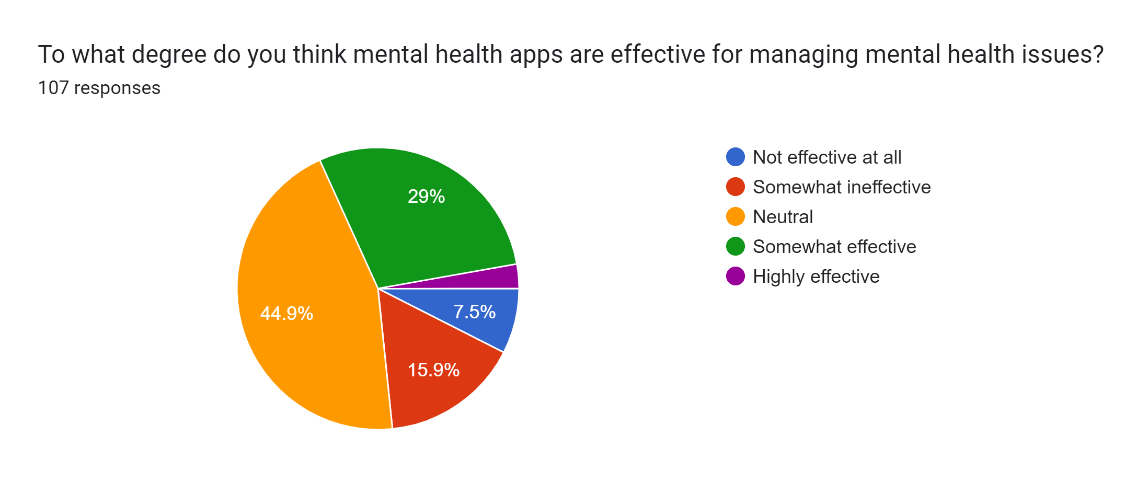
\includegraphics[width=5.2037in,height=2.19079in]{vertopal.com_Survey analysis/vertopal_0d4ab446a1ae41f4824d7f0aaede9ca1/media/image8.png}

The data above is for mapping the perceived efficacy of mental health
apps. Most people have never used a mental health app before, although
during the interviews we realized that a lot of these people might have
used meditation apps or apps that help them with their well-being in
some way. We see this as untapped potential. Especially given that
mental health apps have seen definite growth recently.

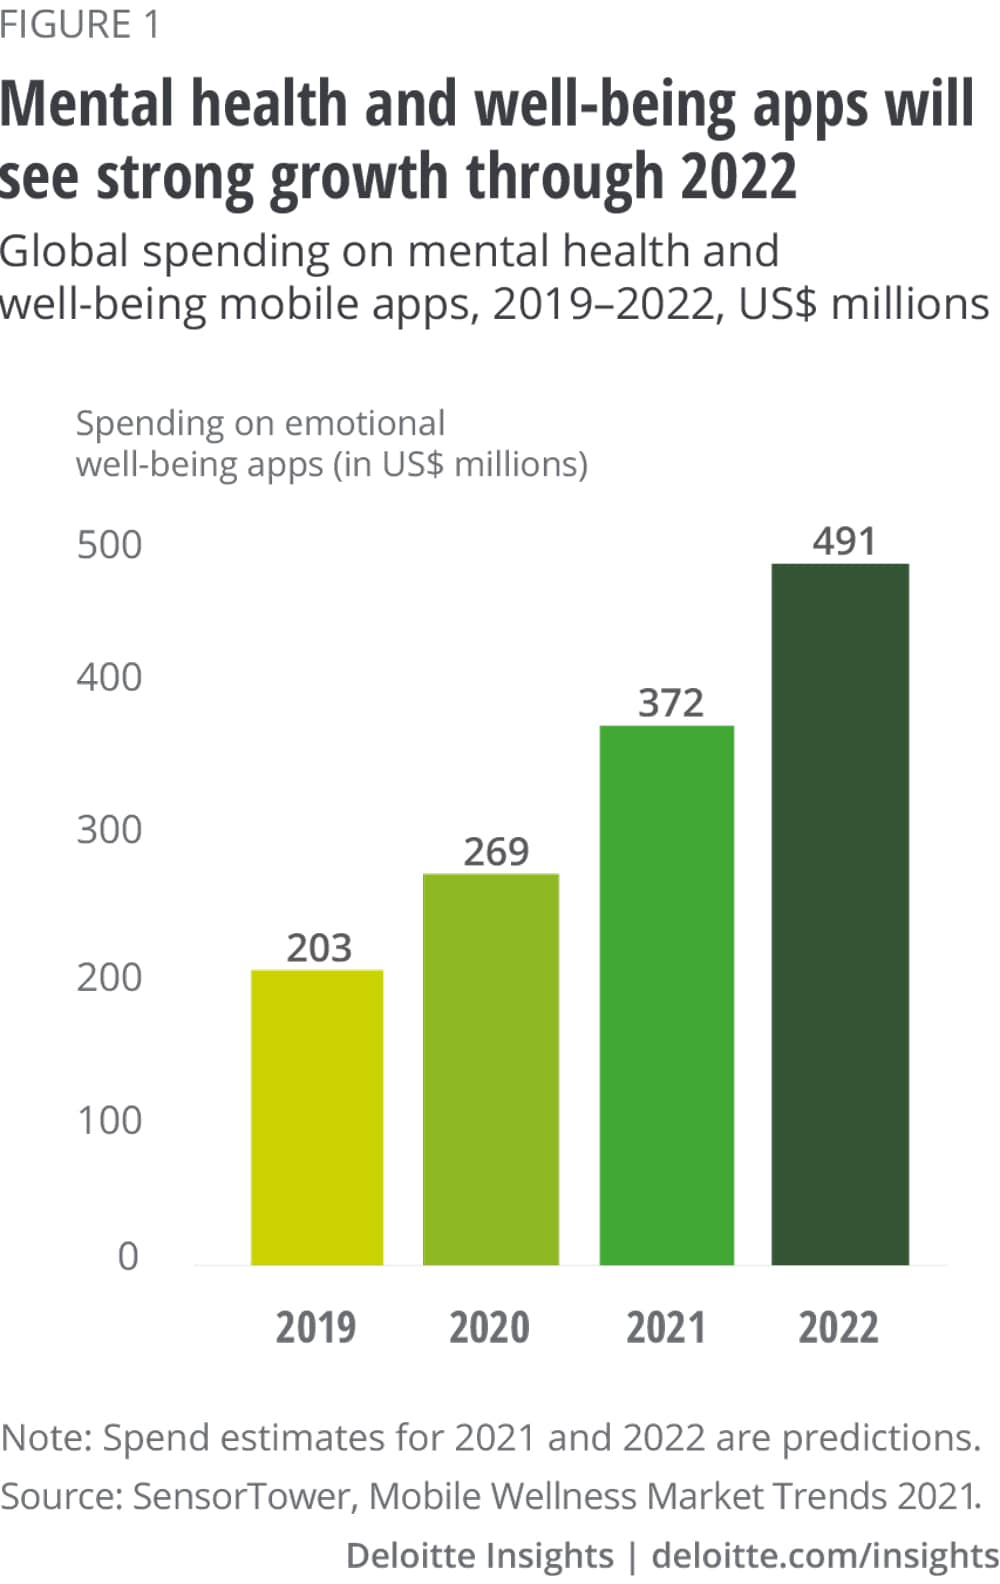
\includegraphics[width=2.82199in,height=4.46997in]{vertopal.com_Survey analysis/vertopal_0d4ab446a1ae41f4824d7f0aaede9ca1/media/image9.jpeg}

``To meet growing demand and capture interested audiences, mental health
app creators and developers can pursue novel methods for monetization,
such as subscription tiers or tailored paid programs and offerings. They
could also explore personalizing these services for users and
customizing apps to encourage regular use and check-ins.''

Source:
\href{https://www2.deloitte.com/us/en/insights/industry/technology/technology-media-and-telecom-predictions/2022/mental-health-app-market.html}{link}

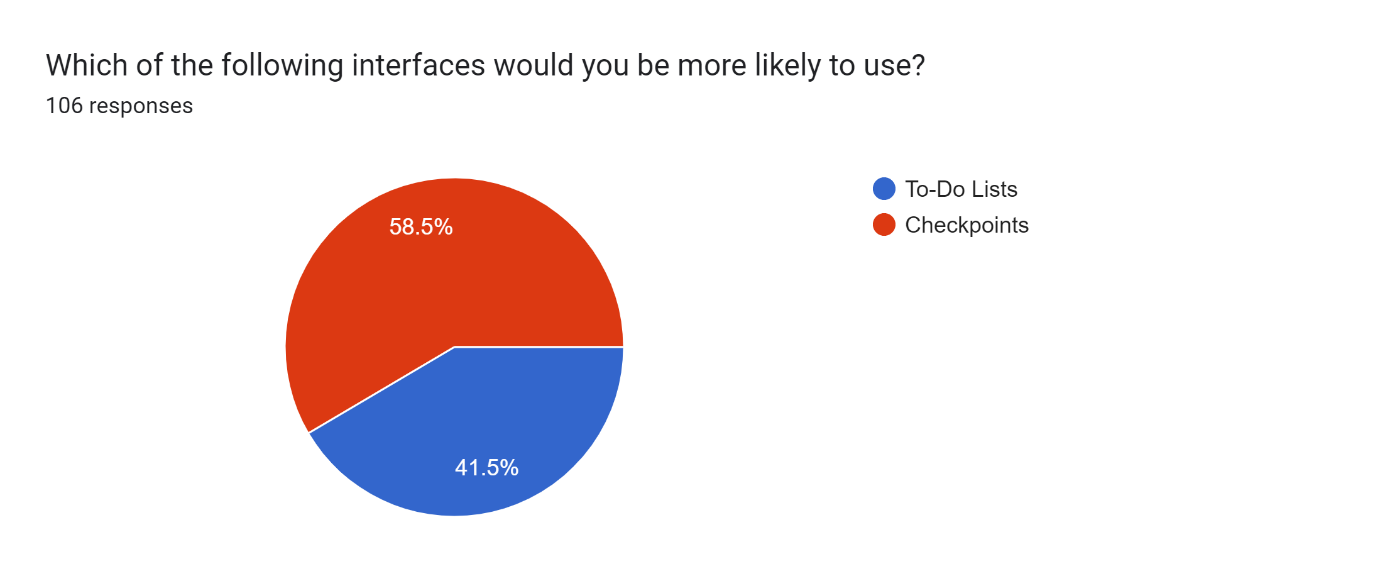
\includegraphics[width=6.26806in,height=2.63889in]{vertopal.com_Survey analysis/vertopal_0d4ab446a1ae41f4824d7f0aaede9ca1/media/image10.png}

We showed the respondents two interfaces. The one with checkpoints was
gamified. This helped us gather that people naturally like gamified
interfaces.

\newpage

\section{Justification of Methods, Processes and Sources}

We adopted a mixed-methods research design to gather insights on the topic. The use of a mixed-methods design enabled us to combine qualitative and quantitative approaches, providing a comprehensive and nuanced understanding of the research problem. A survey via Google Forms was circulated among people. This survey aimed to collect quantitative data on peoples' opinions on mental health and applications used to improve the same. The survey observed 107 responses. We have also carried out interviews with five individuals. The participants were recruited through snowball sampling. The interviews were conducted over Google Meet, and the interview transcripts were further analyzed. The interviewees provided both written and verbal consent for the interview.
\\ \\
Alternative approaches were considered, such as observational and diary studies, but interviews and surveys were selected for their ability to provide in-depth insights into user experiences and preferences.
\\ \\ 
\textbf{Survey} - Considering the standard survey design guidelines, a short and engaging online survey was designed. The survey explored multiple aspects of the topic at hand and the related context, such as the demographics of the participants (two questions), users' knowledge regarding and willingness to seek mental health (three questions), opinions on the use of mental health applications as a tool to improve mental well being (two questions) and user preferences regarding the user interface of the application (one question). Such themes were covered to enable us to establish the background of common user perceptions, challenges, and expectations from an application designed to help people improve their overall mental well-being. The estimated time of completion for the survey was 2-3 minutes, which assisted in preventing participants from avoiding the survey due to an excess of questions. The survey utilized single-select and multiselect options along with textual response fields wherever required, allowing qualitative and quantitative data to be collected. The survey was circulated among university students, working professionals, and other individuals using multiple channels, including private channels and word-of-mouth. Responses to the survey were analyzed and utilized further in the study to gain insights and to frame the interview questions.
\\ \\ 
\textbf{Interviews} - The interviews aimed to comprehend people's mental health needs, challenges, and preferences, providing qualitative insights into their experiences with existing mental health applications and services. Participants were encouraged to share their perspective on what mental health means to them, highlight their experience with any mental health applications, if any and list any features they would like to see in any such app if they were given a chance to use one. They were probed to share their opinions about the motivation behind a person using a mobile application regularly and what they understood by the term 'Gamification'. Semi-structured interviews conducted over Google Meet built upon the research questions established and refined using the initial findings from the survey. The interview maintained the survey's theme while enabling deeper insights due to its personalized, one-on-one nature, overcoming the limitations of the brief survey format. However, the sample population for the interviews lacked diversity, mainly comprising four college students and one school student, potentially introducing bias into the findings. A total of six questions were included in the structure of the interview.
\\ \\
\textbf{Data Analysis} - The interviews were transcribed word-for-word by the team members. This was followed by a Thematic Analysis of the collected data. The survey responses were coded and grouped under themes. The final themes from the surveys and interviews informed our findings and discussion.
\\ \\
\textbf{Literature review} - The literature review was conducted to provide a comprehensive understanding of existing research and knowledge relevant to the development of gamified mental health applications. A systematic search strategy was employed to ensure a thorough review, utilizing Google Scholar as the primary source for looking for relevant literature. The search strategy involved using Boolean expressions to refine search queries and narrow down results. Boolean operators such as "AND," "OR," and "NOT" were used to combine keywords and phrases related to gamification, mental health, user-centered design, and digital health interventions. For example, some of the search queries included combinations like "gamification AND mental health," "user-centered design OR digital health," and "mental health interventions NOT medication." We used Zotero to keep track of all the relevant articles and papers we collected.
\\ \\
Furthermore, papers with high citation counts were prioritized while selecting relevant literature, indicating their influence and relevance. 
In addition, a wide variety of sources were chosen, including journal articles, conference papers, online articles, blog posts, and other relevant sources of information. 
\\ \\
The literature review itself was divided into various stages. We first defined a problem statement for the study, which helped us clearly define the focus and purpose of the literature review. We then identified any themes and patterns from the literature collected. Lastly, we broadly divided the review into five parts: the introduction, the problem, the evidence, the solution and the conclusion. Each section served a specific purpose, facilitating a comprehensive evaluation of existing knowledge and informing the development of the gamified mental health application.

\section{Evaluation Plan}
\begin{enumerate}
    \item \textbf{End Goal:}
    \begin{itemize}
        \item The end goal of the project is to improve users' mental well-being by providing accessible, engaging, and effective mental health support through a gamified app that offers therapy sessions (both online and offline).
        
    \end{itemize}
    \item \textbf{Evaluation Metrics:}
    \begin{itemize}
        \item Gamification Effectiveness: Assessing the effectiveness of gamification features in promoting positive behaviors and mental wellness. Tracking metrics such as completion rates for gamified challenges, user feedback on gamification elements, and changes in user behavior over time.
        \item Measuring user satisfaction with the app and therapy services through surveys, ratings, and reviews. Gathering qualitative feedback on user experiences, perceived benefits, and areas for improvement.
        \item Retention and Long-Term Engagement: Monitoring whether users continue to use the app and engage in therapy sessions over an extended period.

    \end{itemize}
\end{enumerate}
\section{Timeline and approach}

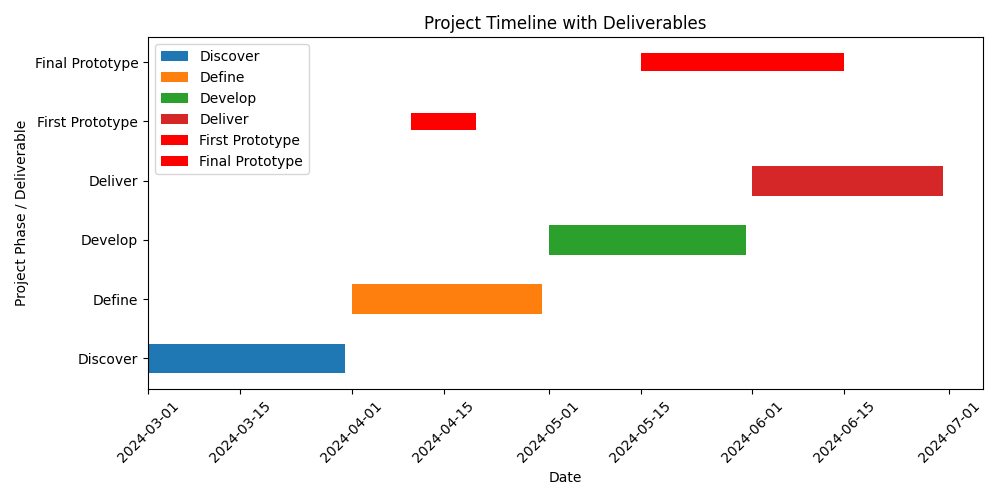
\includegraphics[width=6.26806in,height=2.63889in]{gantt chart.png}

\section{Contributions}
Shamik sinha: Motivation, literature review, patents and concepts, gantt chart, justification
\newline
Tejus: Problem statement, vision, interviews, surveys, analysis, requirement gathering, personas
\newline
Vaibhav: proof of significance, abstract, PACT framework, competitive analysis, evaluation plan


%% The next two lines define the bibliography style to be used, and
%% the bibliography file.
\bibliographystyle{ACM-Reference-Format}
\bibliography{sample-base}

%%
%% If your work has an appendix, this is the place to put it.
\appendix


\end{document}
\endinput
%%
%% End of file `sample-manuscript.tex'.
